\documentclass{article}
\usepackage{lmodern}
\usepackage[T1]{fontenc}
\usepackage{array}
\usepackage{hyperref}
\usepackage{Sweave}
\usepackage[svgnames]{xcolor}
\usepackage{listings}
\lstset{ 
  language=R,
  %%basicstyle=\ttfamily     %doesnt work
  numberstyle=\tiny\color{pink}
  backgroundcolor=\color{white},
  showspaces=false,
  showstringspaces=false,
  showtabs=false,
  rulecolor=\color{black},
  tabsize=2,
  captionpos=b,
  breaklines=true,
  breakatwhitespace=false,
  keywordstyle=\color{teal},      % keyword style
  commentstyle=\color{purple},   % comment style
  stringstyle=\color{orange}      % string literal style
} 

\usepackage{xcolor}
\usepackage{graphicx,subfig}
\graphicspath{ {images/} } 
%preambulo

\title{Causal inference: how to analyse causal scenarios correctly, and repercusions of a wrong analysis}
\author{Nermina Logo Lendo, Rodrigo Jinez and Inés García Ortiz\\
      Bioinformatics and Computational Biology MSc\\
      Universidad Autónoma de Madrid\\
      2021 - 2022}
\date{January 2022}

\begin{document}
% cuerpo del documento
\maketitle
\tableofcontents
\newpage
\section{Objective}

Causal inference is a key element in statistics. It help us reach valuable conclusions about how do variables relate to one another, and help us make decisions in order to mantain our health, combat disease, adjust habits, etc. The problem comes when data is misinterpreted, and correlation is mistaken by causalty. It is very different to say 'ice cream causes cancer' rather than 'in the same season of the year, both ice cream sales and number of melanoma diagnosis increase'. A wrong conclusion can have serious repercusions, that may go from administrating a wrong treatment to ruining the ice cream economy. Even if our field of study is not statistics, it is interesting to understand some basic concepts to prevent us from being fooled by sensational news and develop the so called 'critical thinking'. \par
The \textbf{objective} of this project is to show what changes when data is modelled in the wrong way and how to interpret it correctly. The code can be accessed from the GitHub repository \href{https://github.com/igarcia17/causal_inference}{Causal inference - GitHub repository} . We recommend to get the code from it, as some updates may not be reflected in this file.\par
Along the document, we will explain basic concepts with examples, vaguely based in real life events. It is present all the code necessary to perform each of the cases.\par
Before starting, it is necessary to mention the \textbf{notation} used. When we simulate the data, it is important to stablich the theoretical relation between variables. To talk about the different coefficients, we use the letter 'b', an underscore, and the variables in the direction of the effect. For instance, if we want to set the value of the relation between X and Y, the name of this object will be \(b\_xy\).

\newpage

\section{What to do when there is a common cause}

In this section, we will cover the difficulties that may come when we want to analyse the cause of an outcome variable, Z, when it is affected by X. X is a variable that doesn't only affect Z, but also a second variable, Y: for this reason, X is a \textbf{common cause} of both Z and Y.\par
We have used the following modules to make the analysis:

\begin{lstlisting}

library(dagitty)
library(car)
library(rethinking)
if(!suppressWarnings(require("rethinking", 
quietly = TRUE))) {drawdag <- plot}
  
\end{lstlisting}

The variable Y can have an effect on X or not. This gives us two basic scenarios to work on. The first scenario is illustrated in the following DAG:

\begin{lstlisting}

scenario1.DAG <- dagitty("dag {
X -> Y
X -> Z
e_y -> Y
e_z -> Z
}")

coordinates(scenario1.DAG) <- list(x = c(Y = 1, X = 2, Z = 3, e_y = 0.75, e_z = 2.75), y = c(Y = 3, X = 1, Z = 3, e_y = 2.75, e_z = 2.75))

drawdag(scenario1.DAG)

\end{lstlisting}

\begin{figure}[h]
\caption{Scenario 1.A}
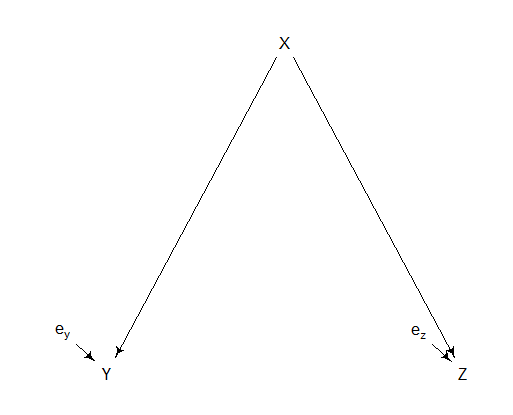
\includegraphics[width=5cm]{scenario1.DAG.png}
\centering
\end{figure}

In this first case, Y is not related to Z.
The second scenario would be:

\begin{lstlisting}
scenario2.DAG <- dagitty("dag {
X -> Y
X -> Z
Y -> Z
e_y -> Y
e_z -> Z}")

coordinates(scenario2.DAG) <- list(x = c(Y = 1, X = 2, Z = 3, e_y = 0.75, e_z = 2.75), y = c(Y = 3, X = 1, Z = 3, e_y = 2.75, e_z = 2.75))

drawdag(scenario2.DAG)
\end{lstlisting}

\begin{figure}[h]
\caption{Scenario 1.B}
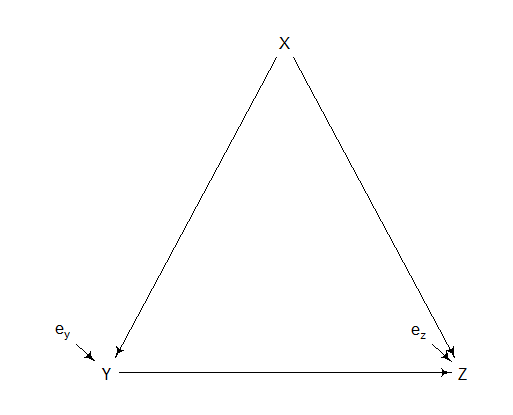
\includegraphics[width=5cm]{scenario2.DAG.png}
\centering
\end{figure}

In this second case, Y does have an effect over Z.\par
It is important to tell the difference between both of them, as the correct model to apply will be different. How can we tell if our data corresponds to one scenario or another?\par
First of all, we have to address one key problem: \textbf{how do we simulate data?}\par
To simulate data in different scenarios, we have used two options: vectors and a function to create datsets. To use vectors is a quick method and very versatile, but if you need to change the coefficients that relate one variable to another it is necessary to create new vectors. Meanwhile, to have a function that creates data frames is useful to make different trials in which the relation between variables is maintained and the coefficients change: the main disadvantage of this method is that anytime the structure of the DAG changes, the function is no longer valid. Both methods are valuable, and each has its advantages and disadvantages. We will use data frames in this chapter and vectors in the next one to show different ways to simulate the data.\par
This first function to create dataframes creates three columns: X, Y and Z. We can change the parameters that relate one varaible to another: if the estimate that multiplies Y for Z is 0, we are representing the scenario 1. \par

\begin{lstlisting}

create.dataset <- function(b_yz, N = 500, b_xy = 3, b_xz = 3,
                           e_x = 1, e_y = 1, e_z = 1) {
  name_df <- data.frame(X = runif(N, 1, 100) + rnorm(N, sd = e_x))
  name_df$Y <- name_df$X * b_xy + rnorm(N, sd = e_y)
  name_df$Z <- name_df$X * b_xz + name_df$Y * b_yz + rnorm(N, sd = e_z)
  return(name_df)}

Ynoinfluences <- create.dataset(0)
Yinfluences <- create.dataset(-2)
non.influences <- create.dataset(0, b_xz = 0)

\end{lstlisting}

Once this is introduce, we can go over the issue that matters. How do we know if our data belongs to scenario 1 or scenario 2? \par

\begin{lstlisting}
Y_check <- function (dataset, conflevel = 0.01) {
  colnames(dataset) <- c('X','Y','Z')
  model_with_Y <- lm(Z~X+Y, data = dataset)
  p.v.X <-(summary(model_with_Y)$coefficients['X','Pr(>|t|)'])
  p.v.Y <- (summary(model_with_Y)$coefficients['Y', 'Pr(>|t|)'])
  
  if ((p.v.X <= conflevel)&(p.v.Y > conflevel))
  {cat("The variable of analysis is not influenced by Y\n")
    cat('See plot\n')
    scenario1.DAG <- dagitty("dag {
    X -> Y
    X -> Z
    e_y -> Y
    e_z -> Z}")
    coordinates(scenario1.DAG) <- list(x = c(Y = 1, X = 2, Z = 3, e_y = 0.75, e_z = 2.75),y = c(Y = 3, X = 1, Z = 3, e_y = 2.75, e_z = 2.75))
    drawdag(scenario1.DAG)
    return(invisible(1))}
  
  if ((p.v.X <= conflevel)&(p.v.Y <= conflevel))
  {cat("The variable of analysis is influenced by both X and Y\n")
    cat('See plot\n')
    scenario2.DAG <- dagitty("dag {
    X -> Y
    X -> Z
    Y -> Z
    e_y -> Y
    e_z -> Z}")
    coordinates(scenario2.DAG) <- list(x = c(Y = 1, X = 2, Z = 3, e_y = 0.75, e_z = 2.75),y = c(Y = 3, X = 1, Z = 3, e_y = 2.75, e_z = 2.75))
    drawdag(scenario2.DAG)
    return(invisible(2))}

  if ((p.v.X > conflevel)&(p.v.Y > conflevel))
  {cat("It seems that neither X or Y affect Z\nYou may want to review your working model\n")
  return(invisible(0))}
  
  if ((p.v.Y <= conflevel)&(p.v.X > conflevel))
  {cat('It looks like Y is related to Z, but not Z\nYou may want to revisit the hypothesis \'X = common cause of Y and Z\'')
  return(invisible(0))}
  }
\end{lstlisting}

An example of its use is:

\begin{lstlisting}
a <- Y_check(non.influences)

## It seems that neither X or Y affect Z
## You may want to review your working model

b <- Y_check(Yinfluences)

##The variable of analysis is influenced by both X and Y
##See plot (scenario2 DAG)
\end{lstlisting}

This function could be optimized in multiple ways, but it shows that the p value of the linear model can be used to classify a data set in one scenario or another. It is necessary to have an idea beforehand of which variable may be the common cause. If by mistake Y is actually the common cause, and X is the mediator, the function wouldn't notice it because \textbf{this couldn't be done by p-values}. This concept, of knowing the 'structure of the DAG' or how variables are related, is crucial in causal inference, and has to be based in real facts. It is similar to which came first, the hen or the egg? Which came first, the melanoma or the exposure to UV radiation?

\subsection{Common casue: scenario 1.A. Descendants of common cause not related}
We will now present a example to illustrate the problems of a bad modelling of scenario 1.A. We will study the expression of gene INK4a, key for melanoma development. It will be the outcome variable, Z. It is directly affected by UV radiation, X. UV radiation can come from sunbathing, which increases the appetite for ice cream consumption, measured in ml of consumed ice cream, Y. You collect data of potentially cancerous tissue from 100 people, from which you know the hours they have spent in the sun the last year, the amount of consumed ice cream and the expression of INK4a.

\begin{lstlisting}
# Theoretical coefficeints between variables
b_xy_i_uv_i <- 5
b_xz_i_uv_i <- 10
b_yz_i_uv_i <- 0
samplesize <- 100

i_uv_i.DAG <- dagitty("dag {
UV.radiation -> Ice.cream.consumption
UV.radiation -> INK4a}")

coordinates(i_uv_i.DAG) <- list(x = c(Ice.cream.consumption = 1, UV.radiation = 2, INK4a = 3),y = c(Ice.cream.consumption = 3, UV.radiation = 1, INK4a = 3))

drawdag(i_uv_i.DAG)
\end{lstlisting}

\begin{figure}[h]
\caption{Scenario 1.A example}
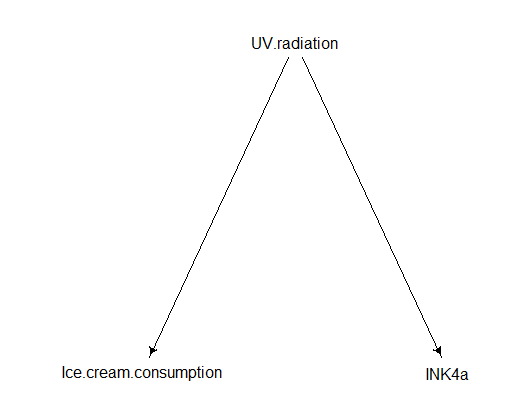
\includegraphics[width=5cm]{i_uv_i.DAG.png}
\centering
\end{figure}

\begin{lstlisting}
sc1.comm <- function(b_yz, N, b_xz, b_xy, reps = 100, ...){
  onlyY_pv <- rep(NA, reps)
  both_pv <- rep(NA,reps)
  onlyX_coefX <- rep(NA,reps)
  both_coefX <- rep(NA, reps)
  
  for (i in 1:reps) {
    dataset <- create.dataset(b_yz, N = N, b_xz = b_xz, b_xy = b_xy, ...)
    
    both <- lm(Z~X+Y, data = dataset)
    onlyY <- lm(Z~Y, data = dataset)
    onlyX <- lm(Z~X, data = dataset)
    onlyY_pv[i] <- summary(onlyY)$coefficients["Y", "Pr(>|t|)"]
    both_pv[i] <- summary(both)$coefficients["Y", "Pr(>|t|)"]
    
    onlyX_coefX[i] <- summary(onlyX)$coefficients["X", "Estimate"]
    both_coefX[i] <- summary(both)$coefficients["X", "Estimate"]
    rm(dataset)}
    
  cat('\n Change in relevance of Y on Z\n')
  cat('\nWhen Z ~ Y: \nThe p value of Y is ', mean(onlyY_pv),'\n')
  cat('\nWhen Z ~Y + X: \nThe p value of Y is ', mean(both_pv), '\n')
  cat('\n Change in effect of X over Z')
  cat('\nWhen Z ~ X: \nThe estimate for X is ', mean(onlyX_coefX),'and its s.d. is', sd(onlyX_coefX),'\n')
  cat('\nWhen Z ~Y + X: \nThe estimate for X is ', mean(both_coefX), 
      'and its s.d. is', sd(both_coefX),'\n')
  cat('\nBeing input x -> z: ', b_xz)
  
  op <- par(mfrow= c(2,1), mar = rep(3,4))
  hist(onlyX_coefX, main = 'Z ~ X', xlab = 'Effect X over Z')
  abline(v = b_xz, col = 'red')
  hist(both_coefX, main = 'Z ~ X + Y', xlab = 'Effect X over Z')
  abline(v = b_xz, col = 'red')
  par(op)}
\end{lstlisting}

If we call this function with the data for this particular case, this is the output: \par

\begin{lstlisting}
sc1.comm(b_yz = b_yz_i_uv_i, N = samplesize, b_xz = b_xz_i_uv_i, b_xy = b_xy_i_uv_i)

## Change in relevance of Y on Z
## When Z ~ Y: 
## The p value of Y is  1.888825e-202 
## When Z ~Y + X: 
## The p value of Y is  0.5211384 
## Change in effect of X over Z
## When Z ~ X: 
## The estimate for X is  10.00005 and its s.d. is 0.003373088 
## When Z ~Y + X: 
## The estimate for X is  9.982808 and its s.d. is 0.444773 
## Being input x -> z:  10
\end{lstlisting}

\begin{figure}[h]
\caption{Frequency of UV radiation estimates over INK4a after 100 repetitions of each model}
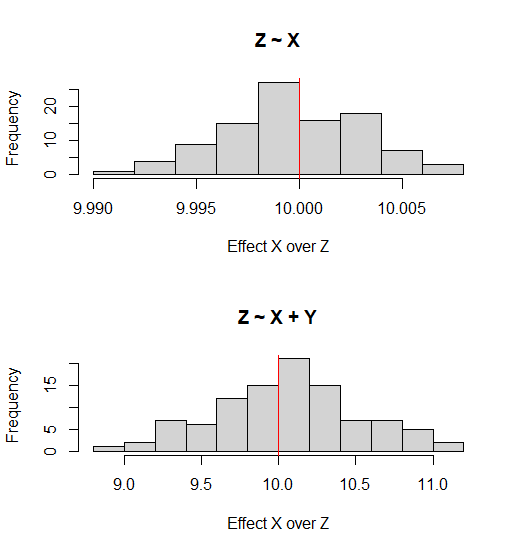
\includegraphics[width=5cm]{i_uv_i1.png}
\centering
\end{figure}

As can be seen, Y is only relevant when we are not condicioning on X. This means that if we condition on ice cream sales but not on UV radiation, we will see association with INK4a. This association is not causation, but if it is mistaken, will result in a quite silly conclusion.

\begin{lstlisting}
impliedConditionalIndependencies(i_uv_i.DAG)
## INK4 _||_ Ic.. | UV.r
\end{lstlisting}

On the other hand, we see that the calculated coefficient for X, thus, UV radiation, is quite similar to the input estimate in both models. What is interesting to see is that the variance of the estimate increases when conditioning on Y.\par
In this type of situation, it is not advised to condition on Y, ice cream, because it won't give more information about melanoma and INK4a and will affect negatively to our estimate of UV radiation, that is a more interesting variable to study. It is important to condition on UV radiation, which is called a \textbf{confounder}.\par

One interesting variation of scenario 1.A, among all variations that can be done, is if there is a variable, A, that is the cause of the confounder. Should we condition on it? Let's see it with the example:\par
\begin{lstlisting}
b_ax_i_uv_i2 <- 2
b_xy_i_uv_i2 <- 5
b_xz_i_uv_i2 <- 10
b_yz_i_uv_i2 <- 0

i_uv_i_sun.DAG <- dagitty("dag {
Sun -> UV.radiation
UV.radiation -> Ice.cream.consumption
UV.radiation -> INK4a}")

coordinates(i_uv_i_sun.DAG) <- list(x=c(Ice.cream.consumption = 1, UV.radiation = 2, Sun = 2, INK4a = 3), y=c(Ice.cream.consumption = 3, UV.radiation = 2, Sun = 1, INK4a = 3))

drawdag(i_uv_i_sun.DAG)
\end{lstlisting}

\begin{figure}[h]
\caption{Scenario 1.A example with ascendant of common cause}
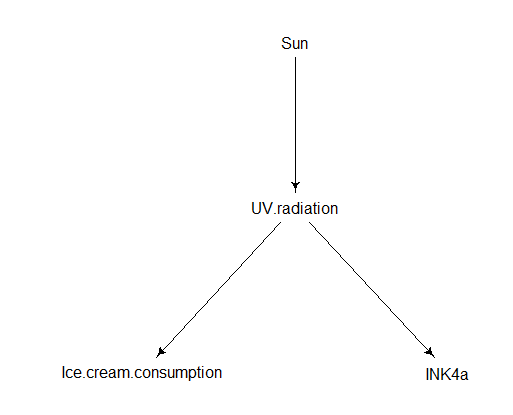
\includegraphics[width=5cm]{i_uv_i_s.DAG.png}
\centering
\end{figure}

As the significance of ice cream, Y, was covered in the previous function, it will be skipped in this one. We are interested in knowing if the sun, A, plays a role in the value of INK4a, Z, and how does it affect X.\par

\begin{lstlisting}
#Necessary to create another function to create a dataset with other structure
create.datasetv2 <- function(b_ax, b_yz=0, N = 500, b_xy = 3, b_xz = 3,
                             e_x = 1, e_y = 1, e_z = 1) {
  name_df <- data.frame(A = runif(N, 1, 100) + rnorm(N))
  name_df$X <- name_df$A * b_ax + rnorm(N, sd = e_x)
  name_df$Y <- name_df$X * b_xy + rnorm(N, sd = e_y)
  name_df$Z <- name_df$X * b_xz + name_df$Y * b_yz + rnorm(N, sd = e_z)
  return(name_df)}
  
sc1.comm.plusancestor <- function(b_yz, N, b_xz, b_xy, b_ax, reps = 30, e_x= 1, ...){
  onlyA_pvA <- rep(NA, reps)
  bothXA_pvA <- rep(NA,reps)
  three_pvA <- rep(NA, reps)
  
  onlyA_coefA <- rep(NA,reps)
  bothXA_coefA <- rep(NA, reps)
  three_coefA <- rep(NA, reps)
  
  onlyX_coefX <- rep(NA,reps)
  bothXA_coefX <- rep(NA, reps)
  three_coefX <- rep(NA, reps)
  
  onlyX_pvX <- rep(NA, reps)
  bothXA_pvX <- rep(NA, reps)
  three_pvX <- rep(NA, reps)
  
  #set.seed(13)
  for (i in 1:reps) {
    dataset <- create.datasetv2(b_yz= b_yz, N = N, b_xz = b_xz, b_ax = b_ax,
                                b_xy = b_xy, e_x =e_x, ...)
    three <- lm(Z~X+A+Y, data = dataset)
    bothXA <- lm(Z~X+A, data = dataset)
    onlyA <- lm(Z~A, data = dataset)
    onlyX <- lm(Z~X, data = dataset)
    
    onlyA_pvA[i] <- summary(onlyA)$coefficients["A", "Pr(>|t|)"]
    bothXA_pvA[i] <- summary(bothXA)$coefficients["A", "Pr(>|t|)"]
    three_pvA[i] <- summary(three)$coefficients["A", "Pr(>|t|)"]
    
    onlyA_coefA[i] <- summary(onlyA)$coefficients["A", 'Estimate']
    bothXA_coefA[i] <- summary(bothXA)$coefficients["A", "Estimate"]
    three_coefA[i] <- summary(three)$coefficients["A", "Estimate"]
    
    onlyX_coefX[i] <- summary(onlyX)$coefficients["X", 'Estimate']
    bothXA_coefX[i] <- summary(bothXA)$coefficients["X", "Estimate"]
    three_coefX[i] <- summary(three)$coefficients["X", "Estimate"]
    
    onlyX_pvX[i] <- summary(onlyX)$coefficients["X", "Pr(>|t|)"]
    bothXA_pvX[i] <- summary(bothXA)$coefficients["X", "Pr(>|t|)"]
    three_pvX[i] <- summary(three)$coefficients["X", "Pr(>|t|)"]
    rm(dataset)}
  
  cat('\n____Change in p value of A on Z\n')
  cat('\nWhen Z ~ A: \nThe p value of A is ', mean(onlyA_pvA),'\n')
  cat('\nWhen Z ~ X + A: \nThe p value of A is ', mean(bothXA_pvA), '\n')
  cat('\nWhen Z ~ Y + X + A: \nThe p value of A is ', mean(three_pvA), '\n')

  cat('\n____Effect of A over Z\n')
  cat('Input A -> X: ', b_ax,'\nInput X -> Z:', b_xz,'\nTotal effect A -> Z', b_xz * b_ax, '\n')
  cat('\nWhen Z ~ A: \nCoefficient of A is ', mean(onlyA_coefA),'and its s.d. is',sd(onlyA_coefA),'\n')
  cat('\nWhen Z ~ X + A: \nCoefficient of A is ', mean(bothXA_coefA),'and its s.d. is',sd(bothXA_coefA),'\n')
  cat('\nWhen Z ~ Y + X + A: \nCoefficient of A is ', mean(three_coefA),'and its s.d. is',sd(three_coefA), '\nSee plots:\n')
  
  op <- par(mfrow= c(2,3))
  hist(onlyA_pvA, main = 'Z ~ A', xlab = 'p value of A')
  hist(bothXA_pvA, main = 'Z ~ X + A', xlab = 'p value of A')
  hist(three_pvA, main='Z ~X + A + Y', xlab = 'p value of A')
  
  hist(onlyA_coefA, main = 'Z ~ A', xlab = 'Effect A over Z')
  abline(v = b_xz*b_ax, col = 'red')
  hist(bothXA_coefA, main = 'Z ~ X + A', xlab = 'Effect A over Z')
  abline(v = b_xz*b_ax, col = 'red')
  hist(three_coefA, main='Z ~X + A + Y', xlab = 'Effect A over Z')
  abline(v = b_xz*b_ax, col = 'red')
  par(op)
  
  #p value of X    ######it is very obvious that it will always have a significant value
  #cat('\n____Change in p value of X on Z\n\nWhen Z ~ A: \nThe p value of X is ', mean(onlyX_pvX),'\n\nWhen Z ~ X +A: \nThe p value of X is ', mean(bothXA_pvX), '\n\nWhen Z ~ Y + X + A: \nThe p value of X is ', mean(three_pvX), '\n')
  
  cat('\n____Effect of X over Z\n\n')
  cat('Input X -> Z: ', b_xz,'\n')
  cat('\nWhen Z ~ A: \nCoefficient of X is ', mean(onlyX_coefX),'and its s.d. is',sd(onlyX_coefX),'\n')
  cat('\nWhen Z ~ X +A: \nCoefficient of X is ', mean(bothXA_coefX),'and its s.d. is', sd(bothXA_coefX),'\n')
  cat('\nWhen Z ~ Y + X + A: \nCoefficient of X is ', mean(three_coefX),'and its s.d. is', sd(three_coefX),'\nSee plots:\n')
  
  op <- par(mfrow= c(2,3))
  hist(onlyX_pvX, main = 'Z ~ X', xlab = 'p value of X')
  hist(bothXA_pvX, main = 'Z ~ X + A', xlab = 'p value of X')
  hist(three_pvX, main='Z ~X + A + Y', xlab = 'p value of X')
  
  hist(onlyX_coefX, main = 'Z ~ X', xlab = 'Effect X over Z')
  abline(v = b_xz, col = 'red')
  hist(bothXA_coefX, main = 'Z ~ X + A', xlab = 'Effect X over Z')
  abline(v = b_xz, col = 'red')
  hist(three_coefX, main='Z ~X + A + Y', xlab = 'Effect X over Z')
  abline(v = b_xz, col = 'red')
  
  par(op)}
\end{lstlisting}

Introducing the data of the problem, the output is:\par

\begin{lstlisting}
sc1.comm.plusancestor(b_yz = b_yz_i_uv_i2, N = samplesize, b_xz=b_xz_i_uv_i2, b_ax = b_ax_i_uv_i2, b_xy = b_xy_i_uv_i2)

#____Change in p value of A on Z
#When Z ~ A: 
#The p value of A is  3.806132e-168 
#When Z ~ X + A: The p value of A is  0.4372251 
#When Z ~ Y + X + A:  The p value of A is  0.4176931 

#____Effect of A over Z
#Input A -> X:  2 
#Input X -> Z: 10 
#Total effect A -> Z 20 
#When Z ~ A: Coefficient of A is  20.00201 and its s.d. is 0.03505331 
#When Z ~ X + A: Coefficient of A is  0.005650556 and its s.d. is 0.2130753 
#When Z ~ Y + X + A: Coefficient of A is  0.005779907 and its s.d. is 0.2167012 
#See plots:
\end{lstlisting}

\begin{figure}[h]
\caption{Histograms of p value and coefficients of Sun (A) over INK4a(Z); data from 30 repetitions of the models}
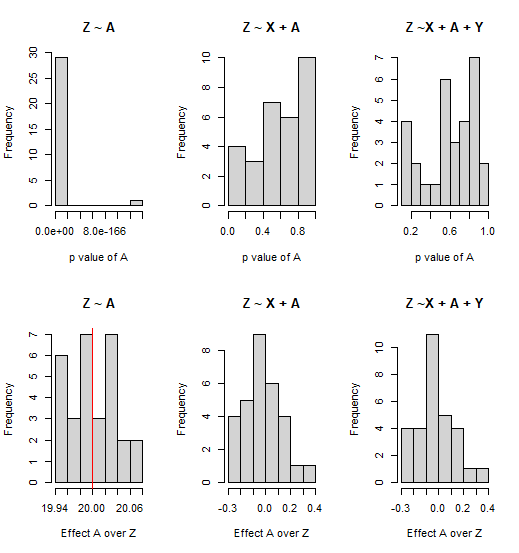
\includegraphics[width=9cm]{histA.sun.png}
\centering
\end{figure}

\begin{lstlisting}
#____Effect of X over Z
#Input X -> Z:  10 
#When Z ~ X: Coefficient of X is  10.00001 and its s.d. is 0.002016263 
#When Z ~ X + A: Coefficient of X is  10.00989 and its s.d. is 0.1031397 
#When Z ~ Y + X + A: Coefficient of X is  10.17693 and its s.d. is 0.5715534 #See plots:
\end{lstlisting}

\begin{figure}[h]
\caption{Histograms of p value and coefficients of UV radiation (X) over INK4a(Z); data from 30 repetitions of the models. Initial error for x = 4}
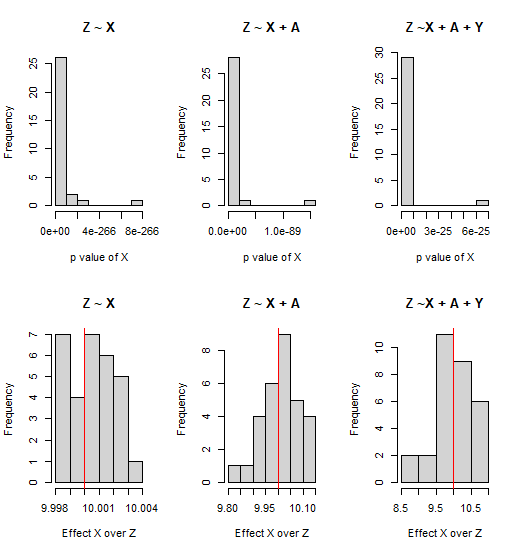
\includegraphics[width=9cm]{histX.sun.png}
\centering
\end{figure} 
\newpage
Let's first talk about A. It only has a significant p value when it is alone in the model, so the coefficients when Z ~ X + A or Z ~ X + A + Y are not relevant. The effect of A on Z can only be appreciated when Z ~ A. This is supported by:

\begin{lstlisting}
impliedConditionalIndependencies(i_uv_i_sun.DAG)
#INK4 _||_ Ic.. | UV.r
#INK4 _||_ Sun | UV.r
#Ic.. _||_ Sun | UV.r
\end{lstlisting}

The p value of X increases with the complexity of the model, but in any case is less significant. The estimate of X is around the expected even if complexity is increased, but its standard error gets higher. In other words, if the cause of study is UV radiation, conditioning on sun is detrimental as the variance of the coefficient increases.\par
As seen in the cause of the cause previous work from Ramon Diaz Uriarte, when the standard error of X increases, the variance of its coefficient when Z ~ X + A is reduced.

\begin{lstlisting}
sc1.comm.plusancestor(b_yz = b_yz_i_uv_i2, N = samplesize, b_xz=b_xz_i_uv_i2, b_ax = b_ax_i_uv_i2, b_xy=b_xy_i_uv_i2, e_x =10)

## When Z ~ X + A: Coefficient of X is  9.999956 and its s.d. is 0.004412072
\end{lstlisting}
\begin{figure}[h]
\caption{Histograms of p value and coefficients of UV radiation (X) over INK4a(Z); data from 30 repetitions of the models. Initial error for x = 40}
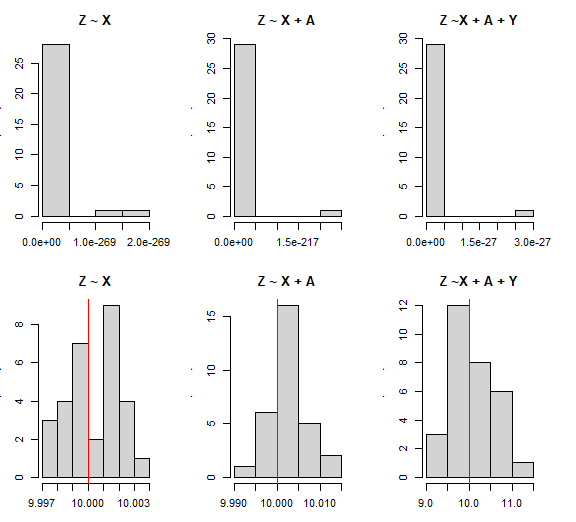
\includegraphics[width=9cm]{sdXdecreased.png}
\centering
\end{figure} 
\newpage

This function also illustrates a key property of causal inference: \textbf{same rules for simple models can be applied to more complex models}.

\subsection{Common casue: scenario 1.B. Descendants of common cause related}

Let's move on to the scenario 1.B. We will illustrate with another example what to expect conditioning on the different possibilities. We have concluded that INK4a overexpression is caused by UV radiation. A recent study shows that there is also intervention of MATP in the French population in this process. It seems to follow the following DAG:\par
\begin{lstlisting}
#Theoretical data
samplesize <- 100
b_xz_m_uv_i <- 4
b_yz_m_uv_i <- (-3)
b_xy_m_uv_i <- 2

m_uv_i.DAG <- dagitty("dag {
UV.radiation -> MATP
UV.radiation -> INK4a
MATP -> INK4a}")

coordinates(m_uv_i.DAG) <- list(x = c(MATP = 1, UV.radiation = 2, INK4a = 3),y = c(MATP = 3, UV.radiation = 1, INK4a = 3))
drawdag(m_uv_i.DAG)
\end{lstlisting}

\begin{figure}[h]
\caption{Example for scenario 1.B}
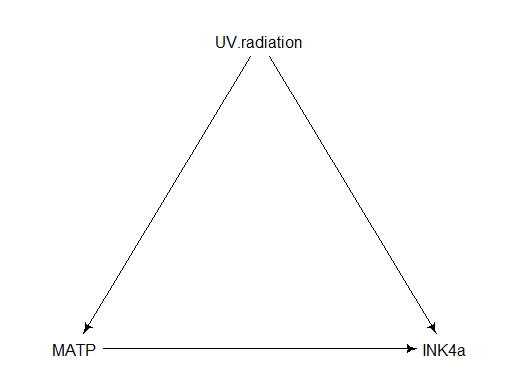
\includegraphics[width=5cm]{m.uv.i.DAG.png}
\centering
\end{figure}

In this case, we are not just asking the question how UV radiation, X, influences INK4a, Z, but we may also be interested in how MATP, Y, affects INK4a.\par
\begin{lstlisting}
sc2.comm <- function(b_xz, b_yz, b_xy, N, reps = 200, ...) {
  onlyY_pvY <- rep(NA, reps)
  both_pvY <- rep(NA, reps)
  onlyX_coefX <- rep(NA,reps)
  both_coefX <- rep(NA, reps)
  onlyY_coefY <- rep(NA,reps)
  both_coefY <- rep(NA,reps)
  
  for (i in 1:reps){
    dataset <- create.dataset(N=N, b_xz = b_xz, b_yz = b_yz, b_xy = b_xy)
    both <- lm(Z~X + Y, dataset)
    onlyY <- lm(Z~Y, dataset)
    onlyX <- lm(Z~X, dataset)
    
    onlyY_pvY[i] <- summary(onlyY)$coefficients['Y', 'Pr(>|t|)']
    both_pvY[i] <- summary(both)$coefficients['Y', 'Pr(>|t|)']
    onlyX_coefX[i] <- summary(onlyX)$coefficients['X', 'Estimate']
    both_coefX[i] <- summary(both)$coefficients['X', 'Estimate']
    onlyY_coefY[i] <- summary(onlyY)$coefficients['Y', 'Estimate']
    both_coefY[i] <- summary(both)$coefficients['Y', 'Estimate']
    rm(dataset)}
  
  cat('p value of Y')
  cat('\nWhen Z~Y:', mean(onlyY_pvY))
  cat('\nWhen Z~Y+X', mean(both_pvY),'\n\n')
  
  cat('___Changes in X\n')
  cat('When Z ~ X:\nX coefficient:', mean(onlyX_coefX), 's.d:', sd(onlyX_coefX))
  cat('\nWhen Z ~ X + Y:\nX coefficient:', mean(both_coefX), 's.d:', sd(both_coefX))
  
  cat('\n\n___Changes in Y\n')
  cat('When Z ~ Y:\nY coefficient:', mean(onlyY_coefY), 's.d:', sd(onlyY_coefY))
  cat('\nWhen Z ~ Y + X:\nY coefficient:', mean(both_coefY), 's.d:', sd(both_coefY))
  
  ##legend: red, direct effect X, blue total effect X, green effect Y
  op <- par(mfrow= c(2,2))
  hist(onlyX_coefX, main = 'Z ~ X', xlab = 'Effect X over Z')
  abline(v = b_xz + b_yz*b_xy, col = 'blue')#total effect, it takes into account both sources of effect
  abline(v = b_xz, col = 'red')#direct effect
  
  hist(both_coefX, main = 'Z ~ X + Y', xlab = 'Effect X over Z')
  abline(v = b_xz + b_yz*b_xy, col = 'blue')#total effect
  abline(v = b_xz, col = 'red')#direct effect
  
  hist(onlyY_coefY, main = 'Z ~ Y', xlab = 'Effect X over Z')
  abline(v = b_yz, col = 'green')
  hist(both_coefY, main = 'Z ~ Y + X', xlab = 'Effect X over Z')
  abline(v = b_yz, col = 'green') 
  par(op)}

sc2.comm(b_xz = b_xz_m_uv_i, b_yz = b_yz_m_uv_i, b_xy = b_xy_m_uv_i,
         N = samplesize)

#p value of Y
#When Z~Y: 1.157204e-134
#When Z~Y+X 7.789572e-38 
#___Changes in X
#When Z ~ X: X coefficient: -2.000495 s.d: 0.01156517
#When Z ~ X + Y: X coefficient: 4.008798 s.d: 0.2082812
#___Changes in Y
#When Z ~ Y: Y coefficient: -1.00081 s.d: 0.00404317
#When Z ~ Y + X: Y coefficient: -3.004562 s.d: 0.1041344
\end{lstlisting}
\begin{figure}[h]
\caption{Estimates of UV radiation and MATP over INK4a}
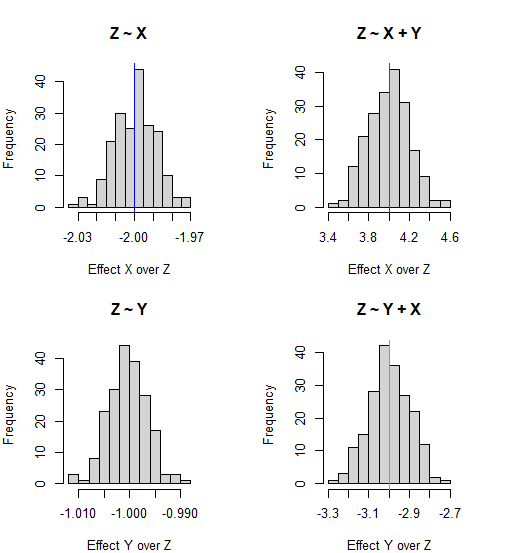
\includegraphics[width=6cm]{histsc2.png}
\centering
\end{figure}

In this case MATP, Y, has a significant p value in both models, in presence and absence of the common cause X, UV radiation. This makes sense and was expected.\par
On blue it is shown the total effect of X over Z, as it takes into account the effect of X over Y as well. On red, it is shown the direct effect of X over Z. On green, the effect of Y over Z.\par
When the mediator Y is out of the model, the X estimates the total effect over Z, including Y contribution. Only when Y is included it is possible to discern what is the direct effect of X. Depending on the case it would be more interesting to study the total or the direct effect of X. For this case, we argue that to know the total effect would be better because in the human body MATP expression is unavoidable. In any case, when there are two covariates in the model the variance of the estimates increase.\par
To know the effect of Y over Z, X has to be taken into account. When UV radiation is not considered, the estimate for MATP is biased; for this reason in this kind of causal structures X is called a confounder, as in the scenario 1. \par
To condition on Y or not may give unexpected outcomes when looking at X over Z. In this case, if MATP is not considered, it seems that the total effect is negative.\par
If we input a higher X->Z value:\par
\begin{lstlisting}
when_xz_4 <- create.dataset(b_xz = b_xz_m_uv_i, b_yz = b_yz_m_uv_i, b_xy = b_xy_m_uv_i,N = samplesize)
scatterplot(Z~X, data = when_xz_4, main ='Original case', regLine=TRUE)
\end{lstlisting}

\begin{figure}[h]
\caption{Variation of INK4a with UV radiation. b\_xz \= 4}
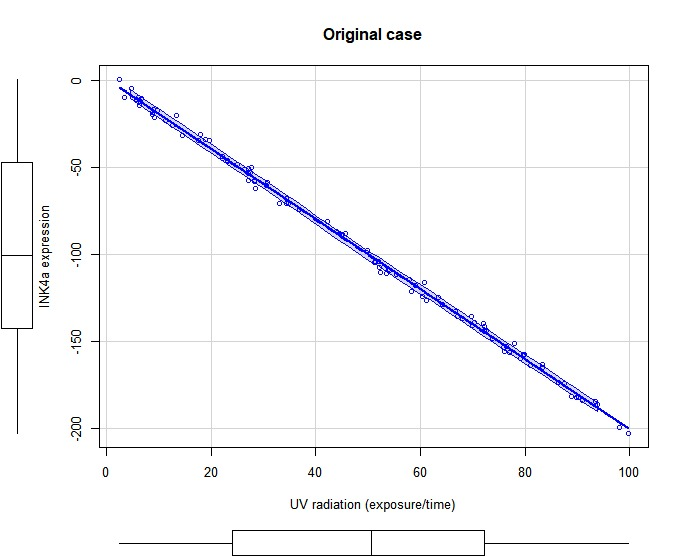
\includegraphics[width=7cm]{scatterplotOriginal.jpeg}
\centering
\end{figure}
\begin{lstlisting}
sc2.comm(b_xz = b_xz_m_uv_i*10, b_yz = b_yz_m_uv_i, b_xy = b_xy_m_uv_i, N = samplesize)

when_xz_40 <- create.dataset(b_xz = b_xz_m_uv_i*10, b_yz = b_yz_m_uv_i, b_xy = b_xy_m_uv_i, N = samplesize)

scatterplot(Z~X, data = when_xz_40, main = 'If UV radiation effect is stronger', regLine=TRUE)

#p value of Y
#When Z~Y: 1.620428e-161
#When Z~Y+X 2.566037e-43 
#___Changes in X
#When Z ~ X: X coefficient: 34.00068 s.d: 0.01156865
#When Z ~ X + Y: X coefficient: 39.99528 s.d: 0.2036934
#___Changes in Y
#When Z ~ Y: Y coefficient: 16.99545 s.d: 0.03612757
#When Z ~ Y + X: Y coefficient: -2.997494 s.d: 0.1018777
\end{lstlisting}

\begin{figure}[h]
\caption{Estimates of UV radiation and MATP over INK4a when b\_xz \= 40}
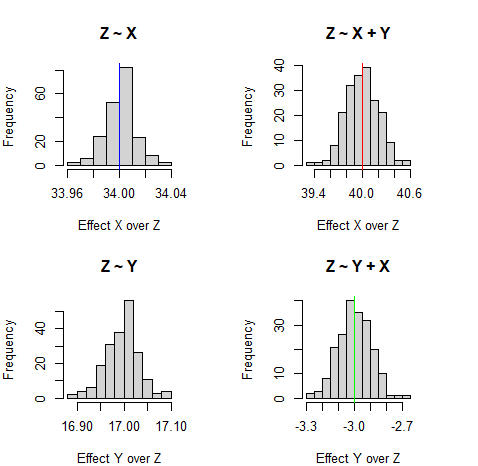
\includegraphics[width=6cm]{hist40.png}
\centering
\end{figure}

\begin{figure}[h]
\caption{Variation of INK4a with UV radiation. b\_xz\=40}
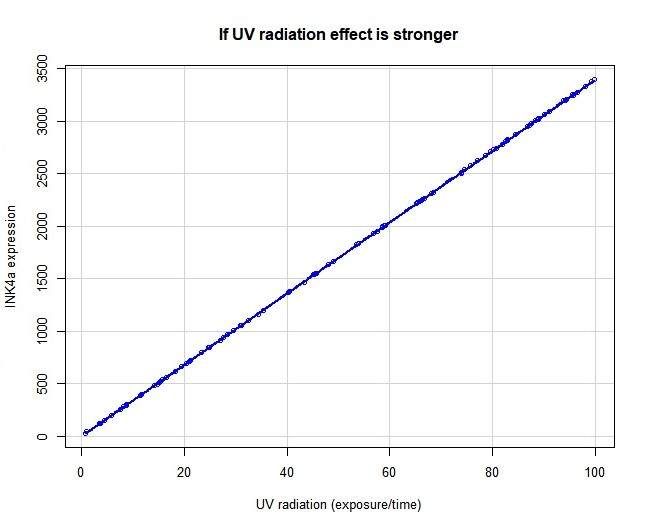
\includegraphics[width=6cm]{scatterplotradiationHIGH.jpeg}
\centering
\end{figure}

This is because the X contribution has a higher impact over Z than Y in this second case. The estimate for X in the simpler model isn't negative, it's total effect is lower than the direct effect. If the Y -> Z value wasn't negative:

\begin{lstlisting}
sc2.comm(b_xz = b_xz_m_uv_i*10, b_yz = b_yz_m_uv_i*(-1), b_xy = b_xy_m_uv_i, N = samplesize)
when_xz_40andnegative <- create.dataset(b_xz = b_xz_m_uv_i*10, b_yz = b_yz_m_uv_i*(-1), b_xy = b_xy_m_uv_i,N = samplesize)
scatterplot(Z~X, data = when_xz_40andnegative, main = 'If MATP enhances INK4a', regLine=TRUE)
#p value of Y
#When Z~Y: 2.258331e-173
#When Z~Y+X 1.924975e-41 
#___Changes in X
#When Z ~ X: X coefficient: 46.00096 s.d: 0.0106993
#When Z ~ X + Y: X coefficient: 40.03247 s.d: 0.213261

#___Changes in Y
#When Z ~ Y: Y coefficient: 22.9915 s.d: 0.03411146
#When Z ~ Y + X: Y coefficient: 2.983863 s.d: 0.1064528
\end{lstlisting}

\begin{figure}[h]
\caption{Estimates of UV radiation and MATP over INK4a when b\_xz \= 40 and b\_yz is positive}
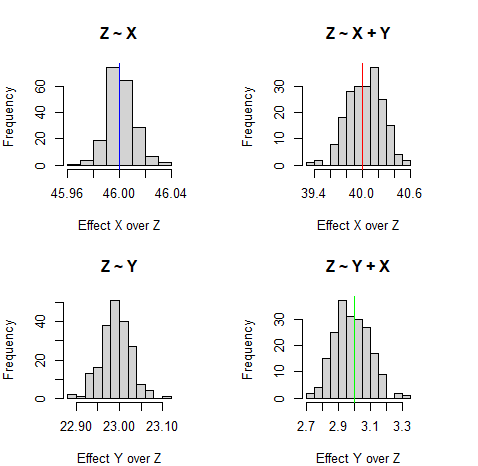
\includegraphics[width=9cm]{hist40neg.png}
\centering
\end{figure}
\newpage
Then the effect of X, UV radiation, over Z, INK4a, is increased, as it should be obvious. \par
The study goes on and we discovers that both the expression of MATP and INK4a is also influenced by another key factor, the cortisol level. This leaves us with the following DAG:\par

\begin{lstlisting}
samplesize <- 100
b_by_m_uv_i_c <- 3
b_bz_m_uv_i_c <- 2
b_xz_m_uv_i_c <- 4
b_xy_m_uv_i_c <- 2
b_yz_m_uv_i_c <- (-3)

m_uv_i_c.DAG <- dagitty("dag {
UV.radiation -> MATP
UV.radiation -> INK4a
Cortisol -> MATP
Cortisol -> INK4a
MATP -> INK4a}")

coordinates(m_uv_i_c.DAG) <- list(x = c(UV.radiation = 1, MATP = 2, INK4a = 2, Cortisol = 3), y = c(UV.radiation = 1, MATP = 2, INK4a = 3, Cortisol = 1))

drawdag(m_uv_i_c.DAG)
\end{lstlisting}

\begin{figure}[h]
\caption{Example scenario 1.B with another common cause more}
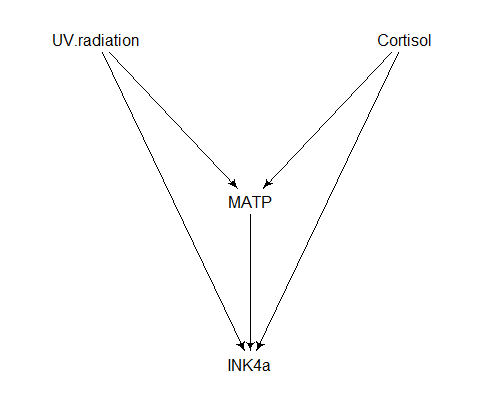
\includegraphics[width=5cm]{mUVicor.png}
\centering
\end{figure}

From the previous function we have learnt that the condition on the mediator variable Y, MATP, would allow us to know the direct effect of UV.radiation. When it is not present in the model, what we can see is the total effect. The reasoning behing the UV.radiation-MATP-INK4a set also apply to the Cortisol-MATP-INK4a set.\par

\begin{lstlisting}
create.datasetv3 <- function(b_by, b_bz, b_yz=(-3), N = 500, b_xy = 3, b_xz = 3, e_x = 1, e_y = 1, e_z = 1, e_b = 1) {
  name_df <- data.frame(B = runif(N, 1, 100) + rnorm(N, sd = e_b))
  name_df$X <- runif(N, 1, 100) + rnorm(N, sd = e_x)
  name_df$Y <- name_df$X * b_xy + name_df$B * b_by +rnorm(N, sd = e_y)
  name_df$Z <- name_df$X * b_xz + name_df$Y * b_yz + 
    name_df$B * b_bz+ rnorm(N, sd = e_z)
  return(name_df)}

sc2.comm.extraoverY <- function(b_by, b_bz, b_xz, b_xy, b_yz, N, reps = 200, ...) { onlyB_coefB <- rep(NA,reps)
  bothBX_coefB <- rep(NA, reps)
  three_coefB <- rep(NA,reps)
  
  for (i in 1:reps){
    dataset <- create.datasetv3(N=N, b_xz = b_xz, b_yz = b_yz, b_xy = b_xy, b_by = b_by, b_bz = b_bz, ...)
    onlyB <- lm(Z ~ B, dataset)
    bothBX <- lm(Z ~ X + B, dataset)
    three <- lm(Z ~ Y + X + B, dataset)
    
    onlyB_coefB[i] <- summary(onlyB)$coefficients['B', 'Estimate']
    bothBX_coefB[i] <- summary(bothBX)$coefficients['B', 'Estimate']
    three_coefB[i] <- summary(three)$coefficients['B', 'Estimate']
    rm(dataset)}

  cat('___Changes in B\n')
  cat('When Z ~ B:\nB coefficient:', mean(onlyB_coefB), 's.d:', sd(onlyB_coefB))
  cat('\nWhen Z ~ X + B:\nB coefficient:', mean(bothBX_coefB), 's.d:', sd(bothBX_coefB))
  cat('\nWhen Z ~ Y + X + B:\nB coefficient:', mean(three_coefB), 's.d:', sd(three_coefB))
  
  #legend: blue, total efffect X, red direct effect X, green effect Y
  op <- par(mfrow= c(1,3), mar = rep(4,4)
  hist(onlyB_coefB, main = 'Z ~ B', xlab = 'Effect B over Z')
  abline(v = b_bz, col = 'red')#direct effect
  abline(v = b_bz + b_yz*b_by, col = 'blue')#total effect of B
  
  hist(bothBX_coefB, main = 'Z ~ B + X', xlab = 'Effect B over Z')
  abline(v = b_bz, col = 'red')#direct effect
  abline(v = b_bz + b_yz*b_by, col = 'blue')#total effect of B
  
  hist(three_coefB, main = 'Z ~ B + X + Y', xlab = 'Effect B over Z')
  abline(v = b_bz, col = 'red')#direct effect
  abline(v = b_bz + b_yz*b_by, col = 'blue')#total effect of B
  par(op)}

sc2.comm.extraoverY(b_by = b_by_m_uv_i_c, b_bz = b_bz_m_uv_i_c,
                     b_xz = b_xz_m_uv_i_c, b_xy = b_xy_m_uv_i_c,
                     b_yz = b_yz_m_uv_i_c, N = samplesize)
#___Changes in B
# When Z ~ B: B coefficient: -6.988085 s.d: 0.1896504
# When Z ~ X + B: B coefficient: -6.999463 s.d: 0.01037498
# When Z ~ Y + X + B: B coefficient: 1.999542 s.d: 0.3236159
\end{lstlisting}

\begin{figure}[h]
\caption{Histogram of estimate of cortisol over INK4a}
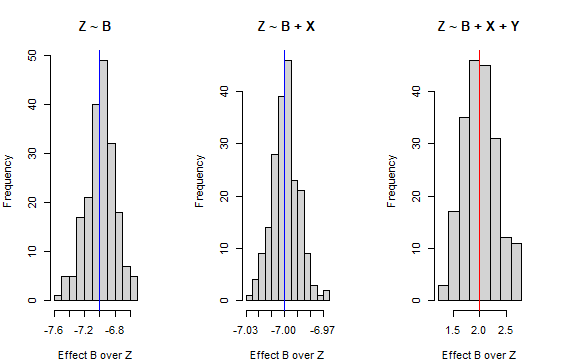
\includegraphics[width=8cm]{histextraoverY.png}
\centering
\end{figure}
As the relation of UV radiation with INK4a is similar to cortisol, we would expect that an histogram of its estimate would be equivalent. The total effect of cortisol, B, is well reflected when it is on its own in the model or when UV radition, X, is considered, because they are independent from each other as can be seen in:\par
\begin{lstlisting}
impliedConditionalIndependencies(m_uv_i_c.DAG)
# Crts _||_ UV.r
\end{lstlisting}

The variance of the coefficient when it is found along X is smaller than when B, cortisol, is checked on its own or when it also considers the collider Y, MATP.\par
Therefore in this type of graph it would be prefered to consider both B and X on the model: the variance of the estimates is smaller and the total effect is calculated. As in the previous case, condiotioning on Y may be counterproductive. \par
The absence of unmeasured confounding for the influence of both the exposure and the intermediate variable on the outcome is required for estimating direct effects. If both of these requirements are not satisfied, no approach can offer unbiased estimates of exposure's direct effects.
This last causal structure introduce us to the next issue: colliders and common effect cases.\par
\newpage

\section{What to do when there is a common effect}

In this second section, we are going to analyze the problems and biases you can create by not controlling a particular case of covariates: the colliders. When studying the effects of differents variables on a particular one, and the  difficulties of adjusting by the collider, Z, when X and Y are its parents and may or may not have an association between them. In this case Z is the \textbf{common effect} of X and Y. We have used the following modules to make the analysis:\par

\begin{lstlisting}

library(dagitty)
if(!suppressWarnings(require("rethinking", 
quietly = TRUE))) {drawdag <- plot}
  
\end{lstlisting}

The variable X can have an effect on Y or not. This gives us two basic scenarios to work on.The first scenario is illustrated in the following DAG:\par

\begin{lstlisting}


comm.effect.DAG <- dagitty("dag {
X -> Z
Y -> Z}")

coordinates(comm.effect.DAG) <- list(x = c(X = 1, Y = 3, Z = 2),y = c(X = 1, Y = 1, Z = 3))

drawdag(comm.effect.DAG)

\end{lstlisting}

\begin{figure}[h]
\caption{Scenario 2.A}
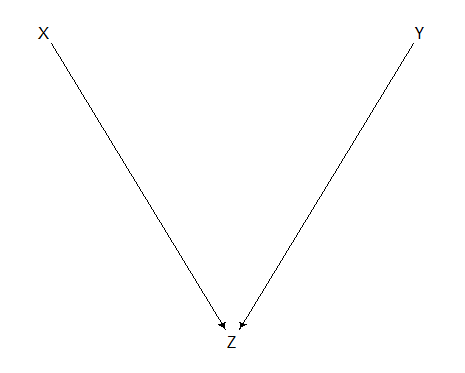
\includegraphics[width=5cm]{comm.effect.DAG.png}
\centering
\end{figure}

For this first case, X is not associated to Y. The second scenario would be:

\begin{lstlisting}

DAG_Situation2 <- dagitty("dag {
X -> Z
Y -> Z
X -> Y}")

coordinates(DAG_Situation2) <- list(x = c(X = 1, Y = 3, Z = 2),y = c(X = 1, Y = 1, Z = 3))

drawdag(DAG_Situation2)
\end{lstlisting}

\begin{figure}[h]
\caption{Scenario 2.B}
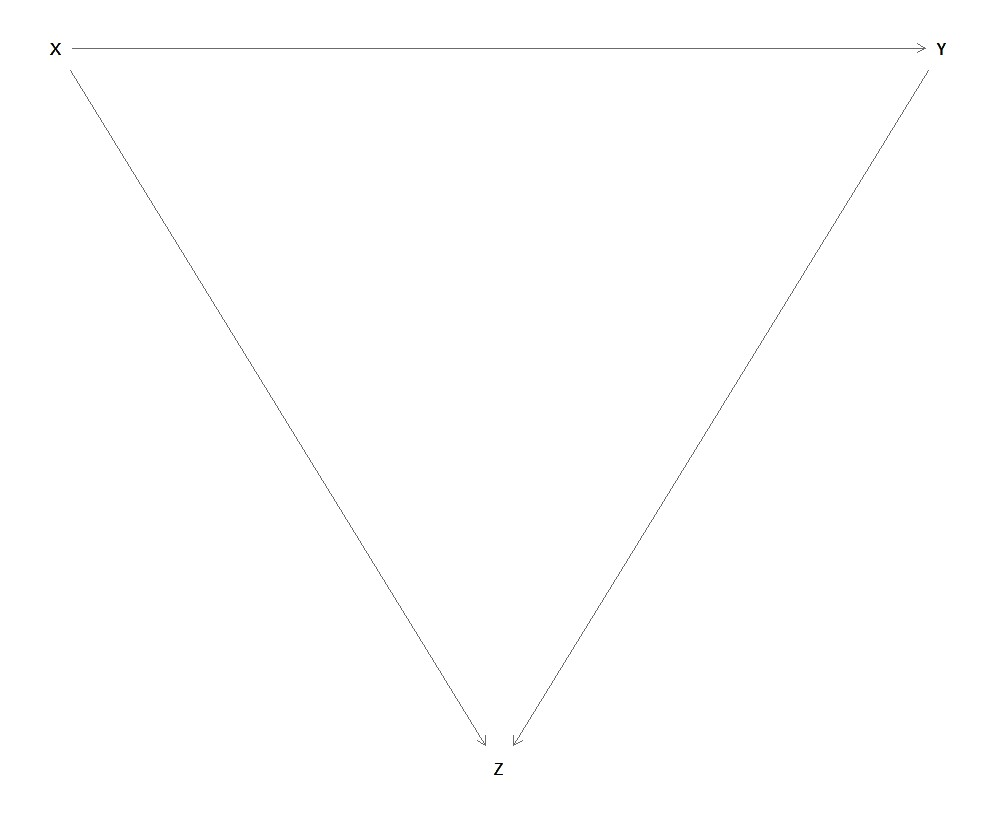
\includegraphics[width=5cm]{DAG_Situation2.png}
\centering
\end{figure}

In this second case, X does have an effect over Y. Whether this two variables do or do not affect each other is important in terms of what kind of effect the adjustment of the collider will have on each one. For the first case, adjusting on the collider will create an association not present before. For the second one, the association between the variables already existed, so what happens is that when we adjust for our collider the direction of that relation might change. \par
For this part, we will simulate our data using vectors. Let's see how we are going to do that for case 1 and case 2.\par

Let us begin with case 2.A:

\begin{lstlisting}

N <- 500
b_xz <- 3
b_yz <- 2
sd_z <- 1

X <- runif(N, 1, 10)
Y <- runif(N, 1.5, 12)
Z <- b_xz * X + b_yz * Y + rnorm(N, 0, sd = sd_z)

\end{lstlisting}

We use vectors to generate random numbers from 1 to 10 for our X variable and from 1.5 to 12 for our Y variable, as both are independent. For our collider (Z) we multiply the values of the two previous variables by a number we want to set as the relation between the parents (X and Y) and the collider (Z). We also add our standard deviation.\par

Now for our case number 2.B:\par

\begin{lstlisting}

b_xy2 <- 1.7 
b_xz2 <- 1.5
b_yz2 <- 2.5

X2 <- runif(N, 1, 10)
Y2 <- X2 * b_xy2 + rnorm(N, mean = 0, sd = 1)
Z2 <- X2 * b_xz2 + Y2 * b_yz2 + rnorm(N, mean = 0, sd = 1)

\end{lstlisting}

In this case there \textbf{is} a relation between X2 and Y2, so for that, we  generate the values for Y2 by multiplying our b\_xy2 and our X values. We  do the same process for the Z2 values as we did for Z in our previous case.\par

Next we will see a function created to generate plots for the regression between two variables, adding our abline. This function will come in handy when we want to check the distribution of our data.\par

\begin{lstlisting}
PLOT.REG <- function(reg_line, plot.var = '') {
  Regres.line <- lm(reg_line)
  plot(reg_line, main = plot.var)
  abline(Regres.line)}

\end{lstlisting}

The function is quite simple, and its manual can be checked in the repository in case more information is needed.\par

\begin{lstlisting}

op <- par(mfrow= c(3, 1))
PLOT.REG(Z ~ X, 'Var distribution X-Z')
PLOT.REG(Z ~ Y, 'Var distribution Y-Z')
PLOT.REG(X ~ Y, 'Var distribution X-Y')
par(op)

\end{lstlisting}

\begin{figure}[h]
\caption{Relation of variables between each other}
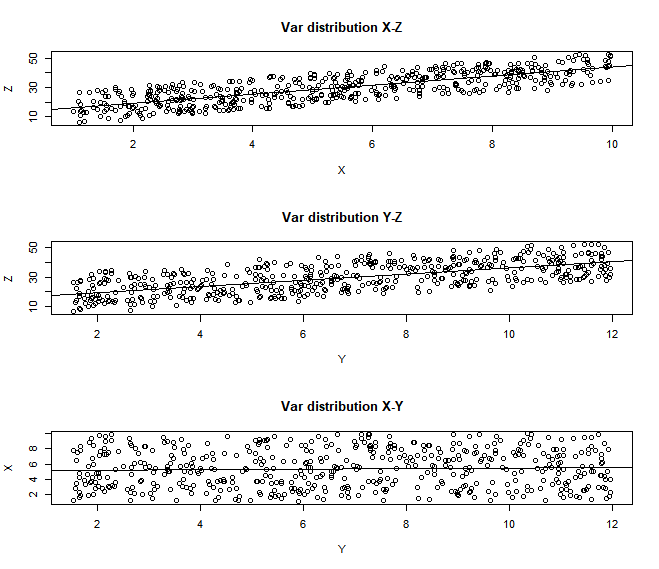
\includegraphics[width=8cm]{PLOT_CASE1.png}
\centering
\end{figure}
\newpage

As we can see, there is, apparently, a positive association between Z and X and also Z and Y. On the other hand, there is no visible association between X and Y  (as should). We can check it by calculating the estimates and significance of each pair. For that we will create a function that accepts the following  arguments: variables to check, dependent variable (to get the estimate and p value), and the title of the variables; the last two ones should be text input in order to make it work.\par
Now that we already checked the distribution of our data, now we should check for our estimates and p values to see if that association or lack thereof is also visible in our values. To do so, we created a function that returns a string that reveals whether there is an association or not, and the values for the estimate and pvalue for our two variables.\par
\begin{lstlisting}

SUM.2VAR <- function(variable1, v_dep1, title_var1, variable2, 
                     v_dep2, title_var2, ...){
  PV1 <- summary(lm(variable1))$coefficients[v_dep1, 'Pr(>|t|)']
  E1 <- summary(lm(variable1))$coefficients[v_dep1, 'Estimate']
  
  PV2 <- summary(lm(variable2))$coefficients[v_dep2, 'Pr(>|t|)']
  E2 <- summary(lm(variable2))$coefficients[v_dep2, 'Estimate']
  
  P.VAL.DICT <- new.env(hash = T, parent = emptyenv())
  assign(title_var1, PV1, P.VAL.DICT)
  assign(title_var2, PV2, P.VAL.DICT)
  
  E.DICT <- new.env(hash = T, parent = emptyenv())
  assign(title_var1, E1, E.DICT)
  assign(title_var2, E2, E.DICT)
  
  for (i in ls(P.VAL.DICT)) {
    if (P.VAL.DICT[[i]] > 0.05)
      cat('The variables', i, 'do not show an association with a p value of',  
          P.VAL.DICT[[i]], 'and an estimate of', E.DICT[[i]], '\n')
    else
      cat('The variables', i, 'show an association with a p value of',  
          P.VAL.DICT[[i]], 'and an estimate of', E.DICT[[i]], '\n')}} 
  # SUMMARY for 2 variables

SUM.3VAR <- function(variable1, v_dep1, title_var1, variable2, 
                     v_dep2, title_var2, variable3, v_dep3, title_var3){
  PV1 <- summary(lm(variable1))$coefficients[v_dep1, 'Pr(>|t|)']
  E1 <- summary(lm(variable1))$coefficients[v_dep1, 'Estimate']
  
  PV2 <- summary(lm(variable2))$coefficients[v_dep2, 'Pr(>|t|)']
  E2 <- summary(lm(variable2))$coefficients[v_dep2, 'Estimate']
  
  PV3 <- summary(lm(variable3))$coefficients[v_dep3, 'Pr(>|t|)']
  E3 <- summary(lm(variable3))$coefficients[v_dep3, 'Estimate']
  
  P.VAL.DICT <- new.env(hash = T, parent = emptyenv())
  assign(title_var1, PV1, P.VAL.DICT)
  assign(title_var2, PV2, P.VAL.DICT)
  assign(title_var3, PV3, P.VAL.DICT)
  
  E.DICT <- new.env(hash = T, parent = emptyenv())
  assign(title_var1, E1, E.DICT)
  assign(title_var2, E2, E.DICT)
  assign(title_var3, E3, E.DICT)
  
  for (i in ls(P.VAL.DICT)) {
    if (P.VAL.DICT[[i]] > 0.05)
      cat('The variables', i, 'do not show an association with a p value of',  
          P.VAL.DICT[[i]], 'and an estimate of', E.DICT[[i]], '\n')
    else
      cat('The variables', i, 'show an association with a p value of',  
          P.VAL.DICT[[i]], 'and an estimate of', E.DICT[[i]], '\n')}
} # SUMMARY for 3 variables

SUM.4VAR <- function(variable1, v_dep1, title_var1, variable2, 
                     v_dep2, title_var2, variable3, v_dep3, title_var3, 
                     variable4, v_dep4, title_var4){
  PV1 <- summary(lm(variable1))$coefficients[v_dep1, 'Pr(>|t|)']
  E1 <- summary(lm(variable1))$coefficients[v_dep1, 'Estimate']
  
  PV2 <- summary(lm(variable2))$coefficients[v_dep2, 'Pr(>|t|)']
  E2 <- summary(lm(variable2))$coefficients[v_dep2, 'Estimate']
  
  PV3 <- summary(lm(variable3))$coefficients[v_dep3, 'Pr(>|t|)']
  E3 <- summary(lm(variable3))$coefficients[v_dep3, 'Estimate']
  
  PV4 <- summary(lm(variable4))$coefficients[v_dep4, 'Pr(>|t|)']
  E4 <- summary(lm(variable4))$coefficients[v_dep4, 'Estimate']
  
  P.VAL.DICT <- new.env(hash = T, parent = emptyenv())
  assign(title_var1, PV1, P.VAL.DICT)
  assign(title_var2, PV2, P.VAL.DICT)
  assign(title_var3, PV3, P.VAL.DICT)
  assign(title_var4, PV4, P.VAL.DICT)
  
  E.DICT <- new.env(hash = T, parent = emptyenv())
  assign(title_var1, E1, E.DICT)
  assign(title_var2, E2, E.DICT)
  assign(title_var3, E3, E.DICT)
  assign(title_var4, E4, E.DICT)
  
  for (i in ls(P.VAL.DICT)) {
    if (P.VAL.DICT[[i]] > 0.05)
      cat('The variables', i, 'do not show an association with a p value of',  
          P.VAL.DICT[[i]], 'and an estimate of', E.DICT[[i]], '\n')
    else
      cat('The variables', i, 'show an association with a p value of',  
          P.VAL.DICT[[i]], 'and an estimate of', E.DICT[[i]], '\n')}
} #SUMMARY for 4 variables

#Let's check our variables:
SUM.4VAR(X ~ Z, "Z", "X and Z", Y ~ Z, "Z", "Y and Z", X ~ Y, "Y", "X and Y", X ~ Y + Z,  "Y", "X and Y (when Z)")
         
#The variables X and Y do not show an association with a p value of 0.3328062 and an #estimate of 0.03488318 
#The variables X and Y (when Z) show an association with a p value of 0 and an estimate of 
#-0.6506454 
#The variables X and Z show an association with a p value of 6.677158e-103 and an estimate #of 0.1942392 
#The variables Y and Z show an association with a p value of 5.433219e-62 and an estimate of #0.2025114

\end{lstlisting}

We can see a strong association between Z and X. There is also a positive relation between Z and Y, but none between X and Y. But the two independent  variables (X and Y) when we adjust by Z raise a association that wasn't supposed to be there.\par
When controling a collider, you can induce a bias in the estimate of theparent variables when there is, actually, none.\par
Knowing now well how to check our estimates and pvalues to aknowledge the association between the two variables (X and Y, whatever those might be), let's explore a more realistic example.\par

\subsection{Common effect: scenario 2.A. Parents are not related}

Here we have a set of variables: cigarettes smoked in a day, COVID19 virus load and \% of lung capacity. Both cigarette consumption and virus load should affect the lung capacity, but there should not be a relation between the number of cigarettes consumed daily and the COV19 virus load.\par

Let's take a look at the DAG:\par

\begin{lstlisting}

DAG.Lung <- dagitty("dag {
cigarettes_day -> lung_capacity
vir_load_COV19 -> lung_capacity
}")

coordinates(DAG.Lung) <- list(x = c(cigarettes_day = 1, vir_load_COV19 = 3, lung_capacity = 2),y = c(cigarettes_day = 1, vir_load_COV19 = 1, lung_capacity = 3))

drawdag(DAG.Lung)
\end{lstlisting}

\begin{figure}[h]
\caption{Example scenario 2.A}
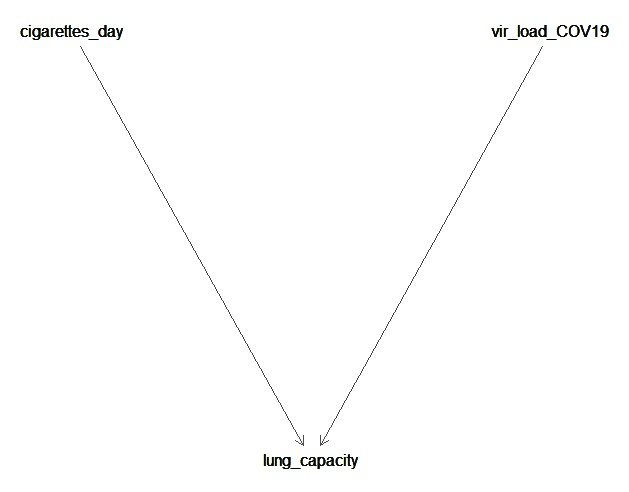
\includegraphics[width=5cm]{DAG_CIG_LUNG.png}
\centering
\end{figure}
We now simulate the data for this particular example, in which both cigarettes and virus load are numerical values, while lung capacity is expressed as a percentage.\par

\begin{lstlisting}

b_cd <- (-0.7) # Relation between cigarettes and lung capacity
b_vlc <- (-0.8) # Relation between virus load and lung capacity 

cigarettes_day <- floor(runif(N, min = 0, max = 45)) #number of cig a day
vir_load_COV19 <- floor(runif(N, min = 0, max = 40)) #Ct
lung_capacity <- 100 + b_cd * cigarettes_day + b_vlc * vir_load_COV19 + 
  rnorm(N, 0, sd = 0.01) #percentage of lung capacity

\end{lstlisting}

Here we have the plots showing the distribution of the variables cigarettes\_day and vir\_load\_COV19, where apparently there is no association and a plot for comparison, cigarettes and lung capacity, with a negative association:\par

\begin{lstlisting}

op <- par(mfrow= c(2, 1))
PLOT.REG(cigarettes_day ~ vir_load_COV19, "Cigarettes ~ Virus_load")
PLOT.REG(cigarettes_day ~ lung_capacity, "Cigarettes ~ Lung_capacity")
par(op)

\end{lstlisting}

\begin{figure}[h]
\caption{Regression of unrelated and related variables}
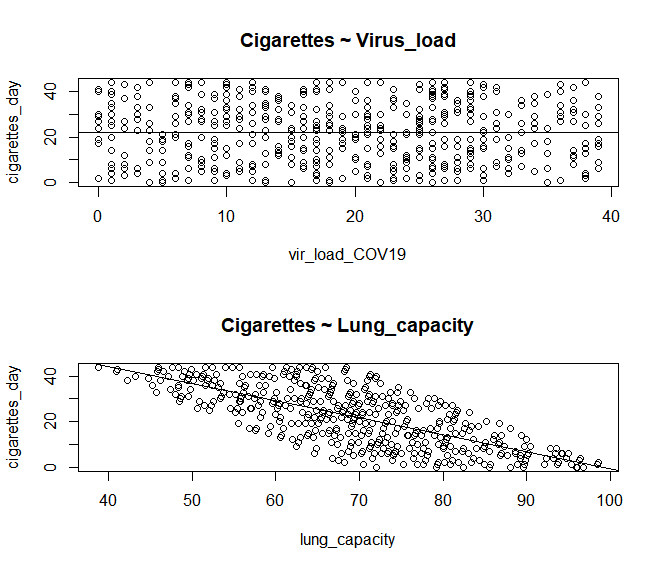
\includegraphics[width=7cm]{PLOT_cig_vir_lung.png}
\centering
\end{figure}

Let's see the relations between our variables.\par

\begin{lstlisting}

SUM.4VAR(cigarettes_day ~ lung_capacity, "lung_capacity", "cigarettes and lung capacity",
         vir_load_COV19 ~ lung_capacity, "lung_capacity", "vir_load_COV19 and lung capacity",
         cigarettes_day ~ vir_load_COV19, "vir_load_COV19", "cigarettes and vir_load_COV19",
          cigarettes_day ~ vir_load_COV19 + lung_capacity, "vir_load_COV19",
         "cigarettes and vir_load_COV19 (when lung capacity)")


#The variables cigarettes and lung capacity show an association with a p value of 3.086284e-83 and an estimate of -0.756362 
#The variables cigarettes and vir_load_COV19 do not show an association with a p value of 0.9486949 and an estimate of -0.003496631 
#The variables cigarettes and vir_load_COV19 (when lung capacity) show an association with a p value of 0 and an estimate of -1.142745 
#The variables vir_load_COV19 and lung capacity show an association with a p value of 1.787942e-70 and an estimate of -0.5881356 

\end{lstlisting}

No association between number of cigarettes smoked a day and the viral load of COV19 infection but a association between these two variables arises when  adjusting for the collider (lung\_capacity).\par
At this point we have already seen how adjusting a collider may create some problems when analyzing data. But things can get a lot more complicated. Let's  not go too far, but see a new example which is a bit more complicated than the previous ones.\par
Imagine we are studying the performance of a professional runner. We have a few variables to take into consideration, but we will focus on the following ones: leg length,metabolism (which affects weight, meaning it also affects performance), heart disease (measured through the values of high-sensitivity cardiac troponin  (hs-cTn)), cholesterol (as a measure of overall health); this last variable  does not affect directly the performance of the runner (speed), but it might through its health. \par
Let's take a look at the DAG:\par

\begin{lstlisting}

DAG.Runner <- dagitty("dag {
cholesterol -> heart
metabolism -> heart
metabolism -> speed
leg_lenght -> speed}")

coordinates(DAG.Runner) <- list(x = c(cholesterol = 1, heart = 3, metabolism = 1, speed = 3, leg_lenght = 1), y = c(cholesterol = 5, heart = 4, metabolism = 3, speed = 2, leg_lenght = 1))
                                       
drawdag(DAG.Runner)

\end{lstlisting}

\begin{figure}[h]
\caption{Complex example of scenario 2.A}
\includegraphics[width=5cm]{DAG_Runner.png}
\centering
\end{figure}

Let's, one more time, generate the data. In this case we have 5 variables, some are associated, others not, it's all on the next piece of code:\par

\begin{lstlisting}

b_ll_s <- 1.2
b_m_s <- 1
b_ch_h <- 0.05
b_m_h <- (-0.3)

leg_lenght <- runif(N, max = 49.75, min = 42.09) #cm
metabolism <- runif(N, 1, 20) 
cholesterol <- runif(N, 125, 200) #mg/dL
speed <- leg_lenght * b_ll_s + metabolism * b_m_s + rnorm(N, mean = 0, sd = 5) #mph
heart <- cholesterol * b_ch_h + metabolism * b_m_h + rnorm(N, mean = 0, sd = 0.1) #ng/L

\end{lstlisting}

Again, let's take a look at the plots for the distribution:\par

\begin{lstlisting}
PLOT.REG(leg_lenght ~ heart, "LEG_LEN ~ HEART")
\end{lstlisting}
\begin{figure}[h]
\caption{Are heart diseases and leg length related?}
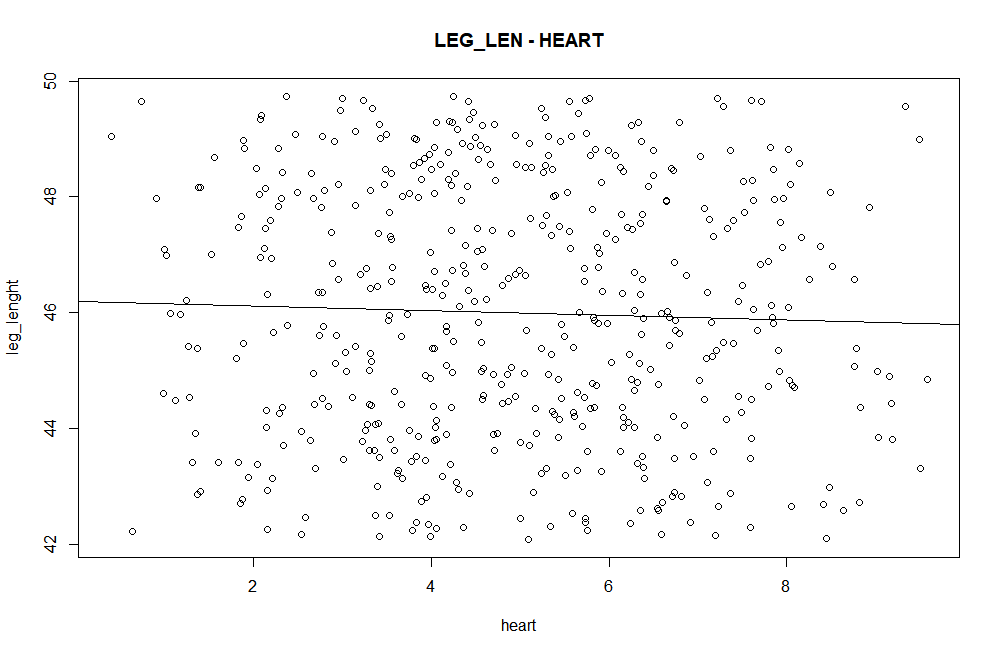
\includegraphics[width=8cm]{PLOT_RUNNER.png}
\centering
\end{figure}

Let's, one more time, check the relations:

\begin{lstlisting}

SUM.4VAR(leg_lenght ~ metabolism, "metabolism", "leg_len and metabolism", leg_lenght ~ cholesterol,
         "cholesterol", "leg_len and cholesterol", leg_lenght ~ heart, "heart", "leg_len and heart", 
         leg_lenght ~ heart + speed, "heart", "leg_len and heart (when speed)")


#The variables leg_len and cholesterol do not show an association with a p value of 0.841257 and an estimate of -0.0009198866 
#The variables leg_len and heart do not show an association with a p value of 0.5383972 and an estimate of 0.0302165 
#The variables leg_len and heart (when speed) show an association with a p value of 3.277156e-12 and an estimate of 0.3962244 
#The variables leg_len and metabolism do not show an association with a p value of 0.3730765 and an estimate of -0.01604611 
\end{lstlisting}
There is no association between leg lenght and metabolism, leg lenght and  cholesterol and leg lenght and heart disease; but when we adjust for the  collider speed, we open a path between leg lenght and heart disease. We  do find  a association between heart when there is no association between  how long your legs are and cardiac disease.\par
Let's look at our data one more time and see whether this association we find when adjusting by our collider (speed) is actually present. The second plot shows the association that actually exists between the variables cholesterol and heart, as opposed to the previous ones (for comparison).\par

\begin{lstlisting}

op <- par(mfrow= c(2, 1))
PLOT.REG(leg_lenght ~ heart, "LEG ~ HEART")

PLOT.REG(cholesterol ~ heart, "CHOLESTEROL ~ HEART")

par(op)
\end{lstlisting}

\begin{figure}[h]
\caption{Relation between heart diseases, leg length and cholesterol}
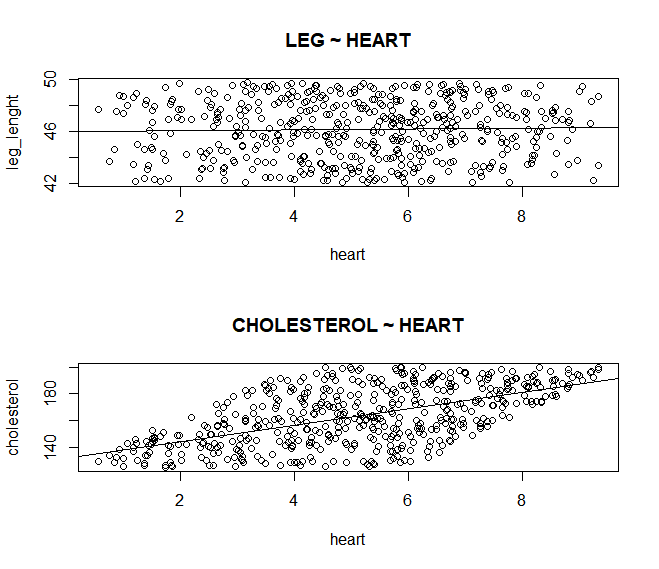
\includegraphics[width=8cm]{COMP_LEG_CHOL_HEART.png}
\centering
\end{figure}
\newpage

\subsection{Common effect: scenario 2.B. Parents are related}

Let's dive in into our second case. In this situation our X and Y variables have some sort of relation but the estimate (its association) changes from positive to negative when we condition on Z (collider).\par

Let's take another peak at the DAG to remind us of the structure:\par

\begin{figure}[h]
\caption{Example of scenario 2.B}
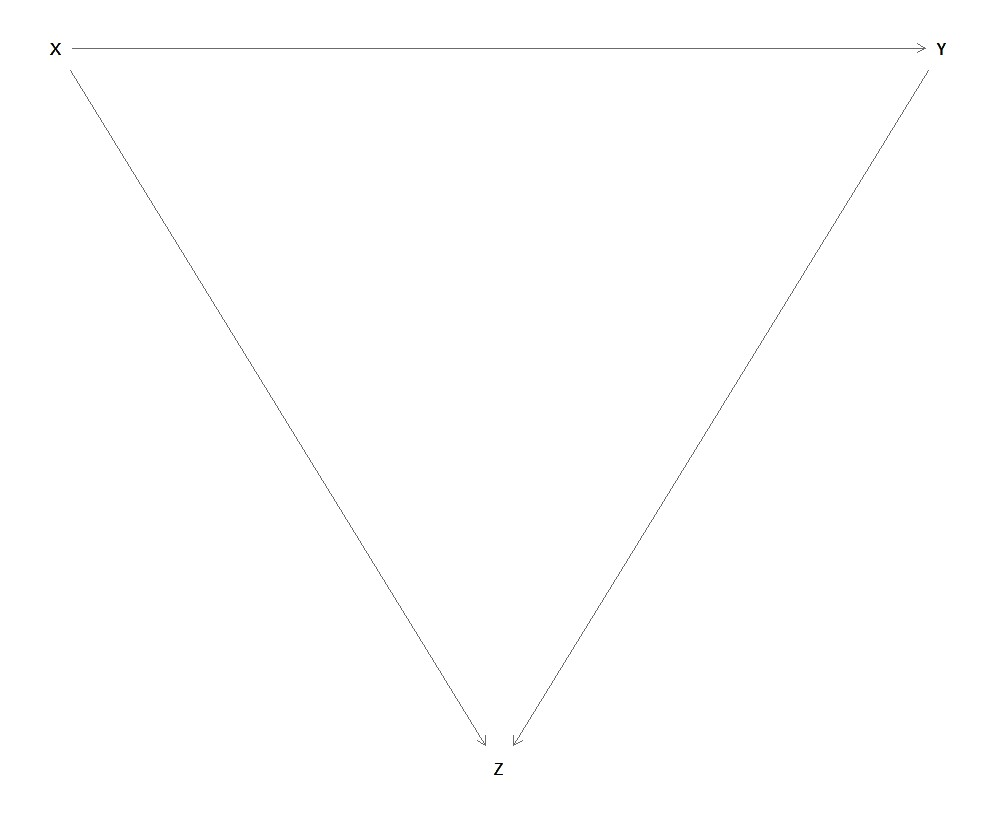
\includegraphics[width=5cm]{DAG_Situation2.png}
\centering
\end{figure}
We, again, generate random data, but in this case the values of Y are associated to the ones from X:\par

\begin{lstlisting}
b_xy2 <- 1.7 
b_xz2 <- 1.5
b_yz2 <- 2.5

X2 <- runif(N, 1, 10)
Y2 <- X2 * b_xz2 + rnorm(N, mean = 0, sd = 1)
Z2 <- X2 * b_xz2 + Y2 * b_yz2 + rnorm(N, mean = 0, sd = 1)
\end{lstlisting}

Let's check our data:\par

\begin{lstlisting}

op <- par(mfrow= c(3, 1))

PLOT.REG(Z2 ~ X2, "Var distribution Z2 ~ X2")
PLOT.REG(Z2 ~ Y2, "Var distribution Z2 ~ Y2")
PLOT.REG(X2 ~ Y2, "Var distribution X2 ~ Y2")

par(op)
\end{lstlisting}

\begin{figure}[h]
\caption{Relation of variables of interset between each other}
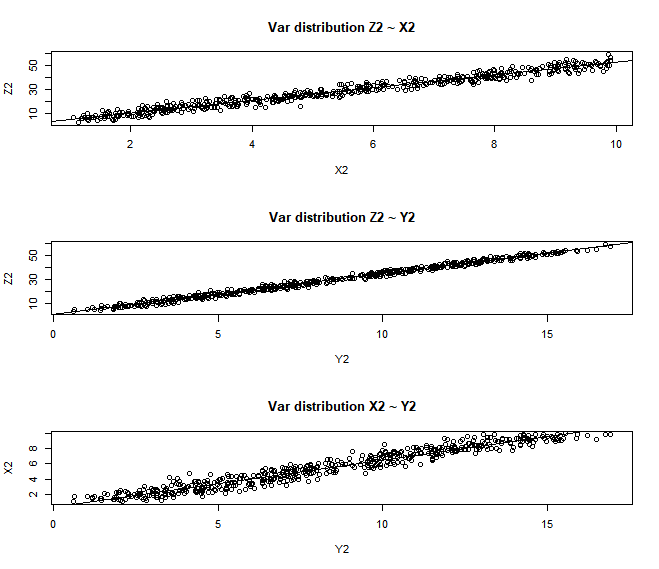
\includegraphics[width=8cm]{PLOT_CASE2.png}
\centering
\end{figure}

As we can see, there is, apparently a positive association between Z2 and X2;  Z2 and Y2; and X2 and Y2. In this case we are interested in the relationship between X2 and Y2; we can check it: \par
\begin{lstlisting}

SUM.2VAR(X2 ~ Y2, "Y2", "X2 and Y2", X2 ~ Y2 + Z2, "Y2", "X2 and Y2 (when Z2)")

#The variables X2 and Y2 show an association with a p value of 1.074789e-301 and an estimate of 0.6174945 
#The variables X2 and Y2 (when Z2) show an association with a p value of 2.690063e-19 and an estimate of -0.4720634 

\end{lstlisting}

The positive association we find between X2 and Y2 switches to a negative association when we adjust for Z2. As we can see, in this particular case, conditioning on Z changes the sign of the estimate for the Y2 variable, as in Simpson's paradox\par


Now, with a more practical example: \par
We want to study the effect of UV radiation (hours of exposure a day) and INK4a on the mutation of gen p53. First of all we illustrate the causal structure:\par

\begin{lstlisting}

DAG.p53 <- dagitty("dag {
UV_radiation -> mutated_p53
INK4a -> mutated_p53
UV_radiation -> INK4a
}")

coordinates(DAG.p53) <- list(x = c(UV_radiation = 1, INK4a = 3, mutated_p53 = 2), y = c(UV_radiation = 1, INK4a = 1, mutated_p53 = 3))
drawdag(DAG.p53)

\end{lstlisting}

\begin{figure}[h]
\caption{Example of scenario 2.B}
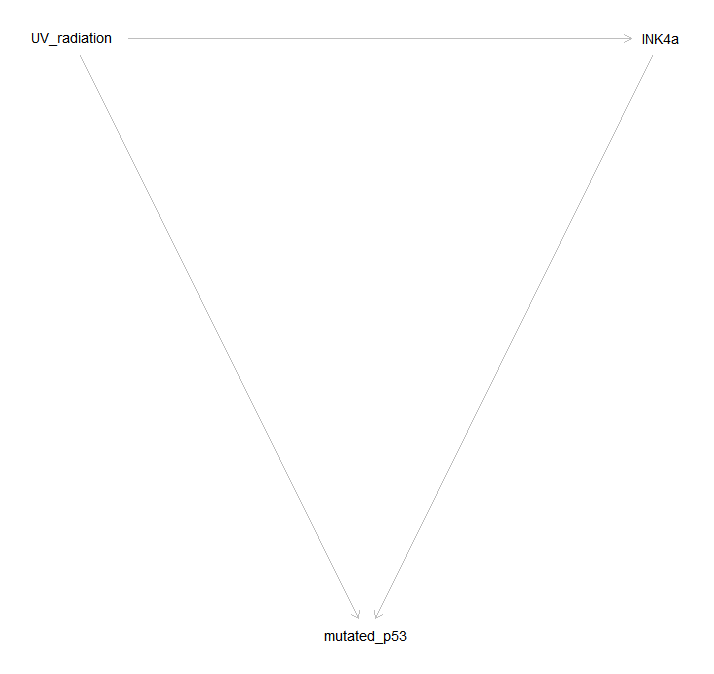
\includegraphics[width=5cm]{DAG_UV_INK_P53.png}
\centering
\end{figure}

Let's generate our data for this particular case:\par

\begin{lstlisting}

b_UV_INK4a <- 0.2
b_INK4a_mp53 <- 2
b_UV_mp53 <- 0.7

UV_radiation <- runif(N, 0, 9)
INK4a <- UV_radiation * b_UV_INK4a + rnorm(N, mean = 0, sd = 0.5)
mutatedp53 <- UV_radiation * b_UV_mp53 + INK4a * b_INK4a_mp53 + rnorm(N, mean = 0, sd = 0.1)
  
\end{lstlisting}

Let's check our data distribution: \par

\begin{lstlisting}

PLOT.REG(UV_radiation ~ INK4a, 'UV ~ INK4a')

\end{lstlisting}

\begin{figure}[h]
\caption{Relation of variables of study}
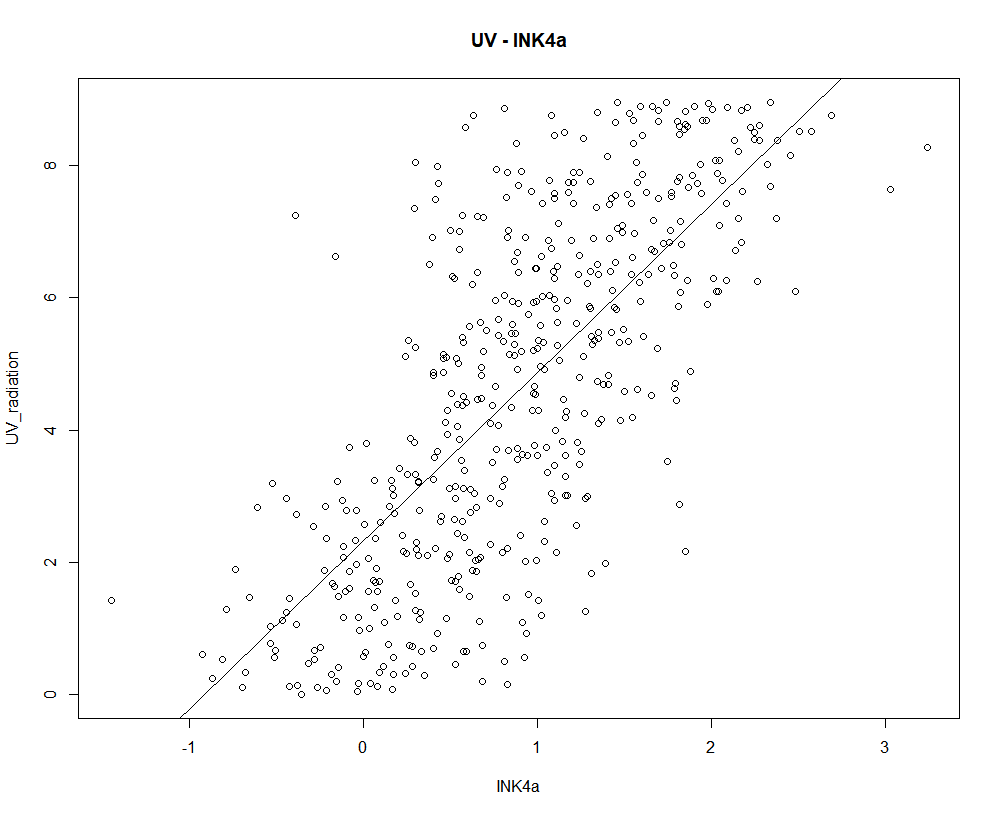
\includegraphics[width=8cm]{PLOT_UV_INK4A.png}
\centering
\end{figure}
We can see a positive association between UV radiation and INK4a.\par

And once again, let's take a look at our models when we adjust for mutated p53 and also when we don't. Does anything change?\par

\begin{lstlisting}

SUM.2VAR(UV_radiation ~ INK4a, "INK4a", "UV and INK4a", UV_radiation ~ INK4a + mutatedp53, "INK4a", "UV and INK4a (when Mp53)")

#The variables UV and INK4a show an association with a p value of 4.878714e-87 and an estimate of 2.647573 
#The variables UV and INK4a (when Mp53) show an association with a p value of 0 and an estimate of -2.81791 

\end{lstlisting}
As shown in the Summary function, the association between the variables UV  radiation is maintained after adjusting for the collider but the relation that was once positive becomes negative when adjusting for Mp53 (collider). Which means, when adjusting for a collider not only we can find an association that isn't supposed to be there but also we can find a change in direction of the association that was previousely present.\par

\subsection{Ancestors and descendants}
Now that we have seen how adjusting the collider can afect the estimates and pvalues, we should also check two more scenarios: Ancestors and Descendants. Let's start with the ancestors.\par
Imagine we have now a variable Z (a collider) that has an ancestor (variable W), does conditioning on any of those two affect the relation between variable X and Y?\par

Let's draw our DAG: 

\begin{lstlisting}

DAG_Ancestor <- dagitty("dag {
X -> Z
Y -> Z
W -> Z}")

coordinates(DAG_Ancestor) <- list(x = c(X = 1, Y = 3, Z = 2, W = 2),y = c(X = 1, Y = 1, Z = 2, W = 3))

drawdag(DAG_Ancestor)
\end{lstlisting}

\begin{figure}[h]
\caption{Case with ancestor extra on collider}
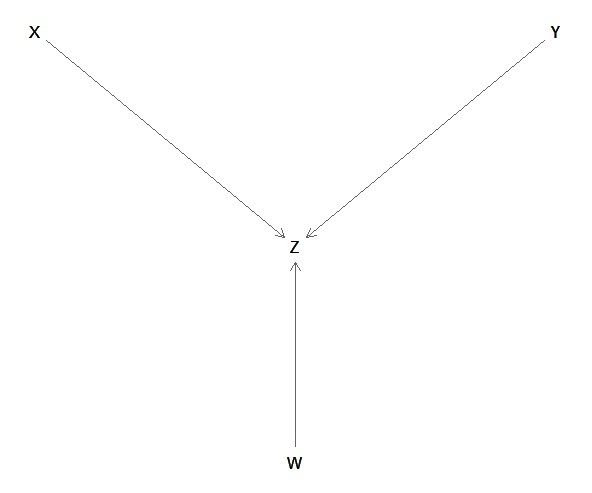
\includegraphics[width=5cm]{DAG_ANCESTOR.png}
\centering
\end{figure}

As always, we create the data according to our DAG:\par

\begin{lstlisting}

b_xz <- 3 
b_yz <- 2
b_wz <- 2.5
sd_z <- 1

X3 <- runif(N, 1, 5)
Y3 <- runif(N, 2, 4)
W3 <- runif(N, 1.5, 3)
Z3 <- b_xz * X3 + b_yz * Y3 + W3 * b_wz + rnorm(N, 0, sd = sd_z)
\end{lstlisting}

And once again we will be checking the summaries for our estimates and pvalues, but this time we want to check also what happens when we adjust for the ancestor of our collider (W).\par

\begin{lstlisting}

SUM.4VAR(X3 ~ W3, "W3", "X3 and W3", X3 ~ W3 + Z3, "W3", "X3 and W3 (when Z3)", X3 ~ Y3 + Z3, "Y3", "X3 and Y3 (when Z3)", X3 ~ Y3, "Y3", "X3 and Y3")

#The variables X3 and W3 show an association with a p value of 0.02225708 and an estimate of 0.2704141 
#The variables X3 and W3 (when Z3) show an association with a p value of 6.253145e-32 and an estimate of -0.6510684 
#The variables X3 and Y3 do not show an association with a p value of 0.7848218 and an estimate of -0.02393977 
#The variables X3 and Y3 (when Z3) show an association with a p value of 1.57704e-41 and an estimate of -0.5242863 
\end{lstlisting}

There is no significant association between X3 and W3, but when conditioned for Z3 a negative association arises. Same thing hapopens between the  variables X3 and Y3. Therefore, conditioning on Z3 modifies the independence between X3, Y3 and W3.\par

\begin{lstlisting}

SUM.2VAR(X3 ~ Y3, "Y3", "X3 and Y3", X3 ~ Y3 + W3, "Y3", "X3 and Y3 (when W3)")

#The variables X3 and Y3 do not show an association with a p value of 0.7848218 and an estimate of -0.02393977 
#The variables X3 and Y3 (when W3) do not show an association with a p value of 0.8489813 and an estimate of -0.01663633 

\end{lstlisting}

No significant association found between X3 and Y3, nor can we find a  association when adjusting for the ancestor (W3). So, conditioning on W3 does not change the independence between X3 and Y3.\par
Let's take a look at a more realistic example: we want to study the effect of cortisol and cholesterol on diabetes, but we also have to take into consideration the variable "sugar consumption in gr". Here is the DAG:

\begin{lstlisting}

DAG.Diabetes.Ancestor <- dagitty("dag {
cortisol -> diabetes
cholesterol -> diabetes
sugar_consumpt -> diabetes}")

coordinates(DAG.Diabetes.Ancestor) <- list(x = c(cortisol = 1, cholesterol = 3,diabetes = 2, sugar_consumpt = 2), y = c(cortisol = 1, cholesterol = 1, diabetes = 2,  sugar_consumpt = 3))
drawdag(DAG.Diabetes.Ancestor)

\end{lstlisting}

\begin{figure}[h]
\caption{Example of ancestor of collider}
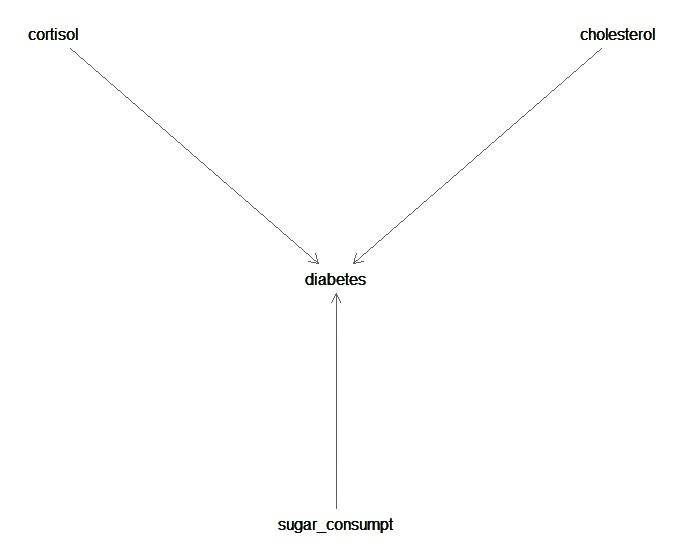
\includegraphics[width=5cm]{DAG_DIAB_ANCESTOR.png}
\centering
\end{figure}

More data...\par

\begin{lstlisting}

b_co_d <- 0.9
b_ch_d <- 0.95
b_sc_d <- 1.2
sd_d <- 1

cortisol <- runif(N, 1, 50)
cholesterol <- runif(N, 10, 250)
diabetes <- cortisol * b_co_d + cholesterol * b_ch_d + sug_consumption * 
  b_sc_d+ rnorm(N, 0, sd = sd_d)
sug_consumption <- runif(N, 0, 150)
\end{lstlisting}

There should not be any association between cortisol and cholesterol. Let's check it on our plot:\par

\begin{lstlisting}

PLOT.REG(cortisol ~ cholesterol, 'cortisol ~ cholesterol')

\end{lstlisting}

\begin{figure}[h]
\caption{Is data associated?}
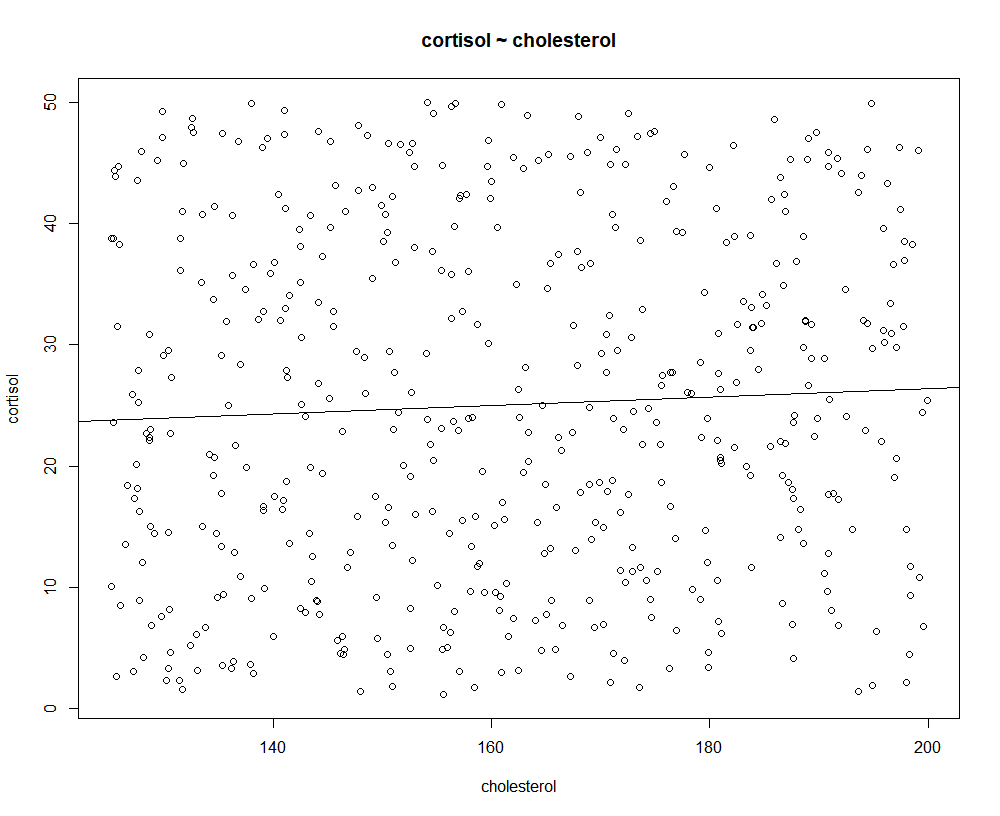
\includegraphics[width=8cm]{PLOT_CORT_CHOL.png}
\centering
\end{figure}

As we can seee, apparently there is no association... But what happens when we adjust for the collider and ancestor?\par

\begin{lstlisting}
SUM.2VAR(cortisol ~ cholesterol, "cholesterol", "cortisol and cholesterol", cortisol ~ cholesterol + sug_consumption, "cholesterol", "colesterol and cortisol (when sugar)")

#The variables colesterol and cortisol (when sugar) do not show an association with a p value of 0.4571814 and an estimate of 0.006613713 
#The variables cortisol and cholesterol do not show an association with a p value of 0.4510984 and an estimate of 0.006693875 

\end{lstlisting}

Again we find no association between cortisol and cholesterol, even if we adjust for the ancestor (sugar\_consumption).\par

\begin{lstlisting}

SUM.2VAR(cortisol ~ cholesterol, "cholesterol", "cortisol and cholesterol", cortisol ~ cholesterol + diabetes, "cholesterol", "colesterol and cortisol (when diabetes)")

#The variables colesterol and cortisol (when diabetes) show an association with a p value of 7.764322e-07 and an estimate of -0.07041942 
#The variables cortisol and cholesterol do not show an association with a p value of 0.4510984 and an estimate of 0.006693875 

\end{lstlisting}

But we do find a association between those two variables when adjusting for diabetes (the collider).\par
Let's take a look at our second possible scenario with the ancestor and descendant situations. We now have a variable Z (a collider) that has a descendant (variable W), does conditioning on any of those two affect the relation between variable X and Y?\par
Starting with the DAG:

\begin{lstlisting}

DAG.Descendant <- dagitty("dag {
X -> Z
Y -> Z
Z -> W
e_z -> Z}")

coordinates(DAG.Descendant) <- list(x = c(X = 1, Y = 3, Z = 2, e_z = 1.75, W = 2),y = c(X = 1, Y = 1, Z = 2, e_z = 2, W = 3))

drawdag(DAG.Descendant)

\end{lstlisting}

\begin{figure}[h]
\caption{Descendant of a collider}
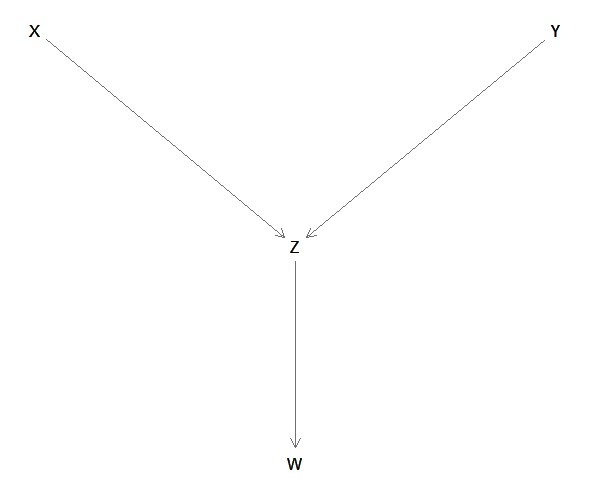
\includegraphics[width=5cm]{DAG_DESCENDANT.png}
\centering
\end{figure}

We generate the data...\par

\begin{lstlisting}
b_xz <- 1.1
b_yz <- 0.7
b_zw <- 2
sd_z <- 0.5
sd_w <- 0.5

X4 <- runif(N, 1, 10)
Y4 <- runif(N, 2, 20)
Z4 <- b_xz * X4 + b_yz * Y4 +  rnorm(N, 0, sd = sd_z)
W4 <- b_zw * Z4 + rnorm(N, 0, sd = sd_w)

\end{lstlisting}

And check our estimates and pvalues once more:\par

\begin{lstlisting}

SUM.3VAR(X4 ~ Y4, "Y4", "X4 and Y4", X4 ~ Y4 + W4, "Y4", "X4 and Y4 (when W4)", X4 ~ Y4 + Z4, "Y4", "X4 and Y4 (when Z4)")

#The variables X4 and Y4 do not show an association with a p value of 0.471942 and an estimate of -0.01698028 
#The variables X4 and Y4 (when W4) show an association with a p value of 8.300303e-322 and an estimate of -0.6199551 
#The variables X4 and Y4 (when Z4) show an association with a p value of 0 and an estimate of -0.6217867 
\end{lstlisting}

We find no association between X4 and Y4, but when we condition on the collider (Z) or its descendant (W4) we find a significantly negative association between the two variables. \par
In this case adjusting by Z4 and W4 (its descendant) resulted in a association between the variables X4 and Y4. \par

\textbf{Practical example:} we want to see how does diabetes affect heart disease for that we will also measure cortisol and cholesterol, which affect diabetes. Let's see what happens when we condition the collider or its descendant in this particular case. First we create the DAG:

\begin{lstlisting}

DAG.Diabetes.Descendant <- dagitty("dag {
cortisol -> diabetes
cholesterol -> diabetes
diabetes -> heart_disease}")

coordinates(DAG.Diabetes.Descendant) <- list(x = c(cortisol = 1, cholesterol = 3, diabetes = 2,heart_disease = 2), y = c(cortisol = 1, cholesterol = 1,diabetes = 2, heart_disease = 3))

drawdag(DAG.Diabetes.Descendant)

\end{lstlisting}

\begin{figure}[h]
\caption{Example of a descendant of a collider}
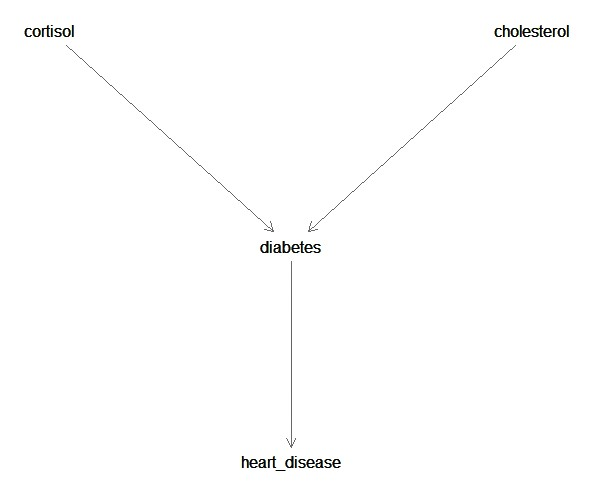
\includegraphics[width=5cm]{DAG_DESCENDANT_DIAB.png}
\centering
\end{figure}

As the example is very simmilar to the previous one, we will be using the same values for the data, excepting the heart disease variable.\par
\begin{lstlisting}
 
b_co_d_d <- 1.5
b_ch_d_d <- 0.95
b_d_hd <- 2.5
sd_d_d <- 5
sd_hd <- 2

cortisol_desc <- runif(N, 1, 50)
cholesterol_desc <- runif(N, 10, 250)
diabetes_desc <- cortisol_desc * b_co_d_d + cholesterol_desc * b_ch_d_d +  rnorm(N, 0, sd = sd_d_d)
heart_disease <- diabetes_desc * b_d_hd + rnorm(N, 0, sd = sd_hd)

\end{lstlisting}

Let's check the values...\par

\begin{lstlisting}

SUM.3VAR(cortisol_desc ~ cholesterol_desc, "cholesterol_desc", "cortisol and cholesterol", cortisol_desc ~ cholesterol_desc + diabetes_desc, "cholesterol_desc", "cortisol and cholesterol (when diabetes)", cortisol_desc ~ cholesterol_desc + heart_disease, "cholesterol_desc", "cortisol and cholesterol (when heart disease)")

#The variables cortisol and cholesterol do not show an association with a p value of 0.424835 and an estimate of -0.007447195 
#The variables cortisol and cholesterol (when diabetes) show an association with a p value of 8.388719e-309 and an estimate of -0.6025828 
#The variables cortisol and cholesterol (when heart disease) show an association with a p value of 1.393365e-304 and an estimate of -0.6017466 

\end{lstlisting}

Just like in our previous simple example, in this case there should not be any relation between cortisol and cholesterol (as we did intend with our data) and when we see our summary we can confirm there is no relation. But when we  condition on our collider or its descendant (heart disease) a association between the variables cortisol and cholesterol arises.\par
To better visualize this non existent association between our two variables we can check the plot for the regression of both of them and it's pretty clear that there is no apparent positive or negative association. To reinforce this data, we can also check and compare the plot for the variables cortisol and heart disease, where we see a positive association.

\begin{lstlisting}

op <- par(mfrow= c(2, 1))
PLOT.REG(cortisol_desc ~ cholesterol_desc, 'cortisol ~ cholesterol')
PLOT.REG(cortisol_desc ~ heart_disease, 'cortisol ~ heart_disease')
par(op)

\end{lstlisting}

\begin{figure}[h]
\caption{Distribution of data plots}
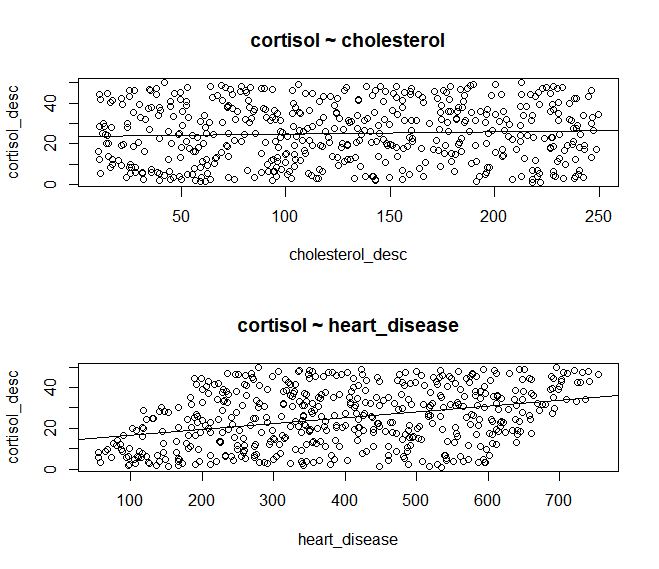
\includegraphics[width=8cm]{PLOT_CR_CH_HD.png}
\centering
\end{figure}

\newpage

\section{Complex cases and backdoor criteria}

To develop this issue, we will need the following packages:

\begin{lstlisting}
library(simstudy)
library(dagitty)
library(rethinking)
if(!suppressWarnings(require("rethinking", quietly = TRUE))) {drawdag <- plot}
\end{lstlisting}

\subsection{Berkson\'s paradox}

A specific collider bias that has a quite famous example (\"Why are handsome men such jerks?\") is the Berkson's paradox. This paradox produces a selection bias, and it is caused by systematically observing some events more than others. Let's explain a little bit of this paradox using the previousely mentioned example:

\begin{figure}[h]
\caption{Selection bias: why are handsome men such jerks?}
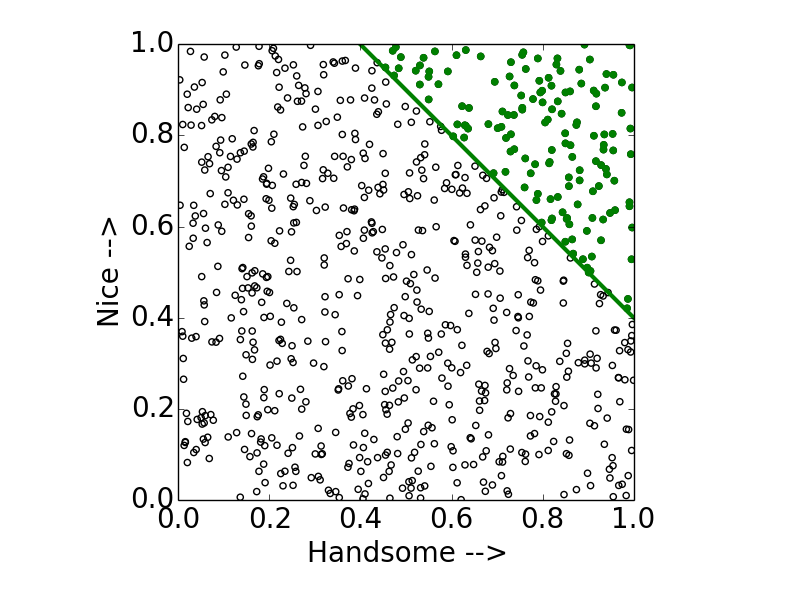
\includegraphics[width=8cm]{berkson_men.png}
\centering
\end{figure}

If we take a look at this plot, we can see that there is no apparent association between being handsome and being nice. The data shows independence between these two variables. But, being a smart woman, you are probably not going to look for an unpleasant man or an ugly one. Your goal is probably somewhere in the green area shown in the plot. But those man might not be single or interested in you so you would probably accept a not so handsome man that is really nice or a not so nice man that is really handsome. And that\'s what causes your bias. You only pay attention to specific groups of population, as you are not even considering man who are not very nice and also not very handsome (which wouldn't be very convenient). This is what Berkson\'s paradox describes, a selection bias in our observations.\par
Okay, now that we know not all handsome man are jerks, let's take a look at a different example.\par
We are going to observe hospital patients with diabetes and hospital patients with cholecystitis.The corresponding DAG:\par

\begin{lstlisting}
DAG.Berkson <- dagitty("dag {
diabetes -> hosp_patient
cholycistitis -> hosp_patient}")

coordinates(DAG.Berkson) <- list(x = c(diabetes = 1,  cholycistitis = 3,hosp_patient = 2),y = c(diabetes = 1, cholycistitis = 1, hosp_patient = 3))

drawdag(DAG.Berkson)
\end{lstlisting}

\begin{figure}[h]
\caption{Example of Bercksons paradox}
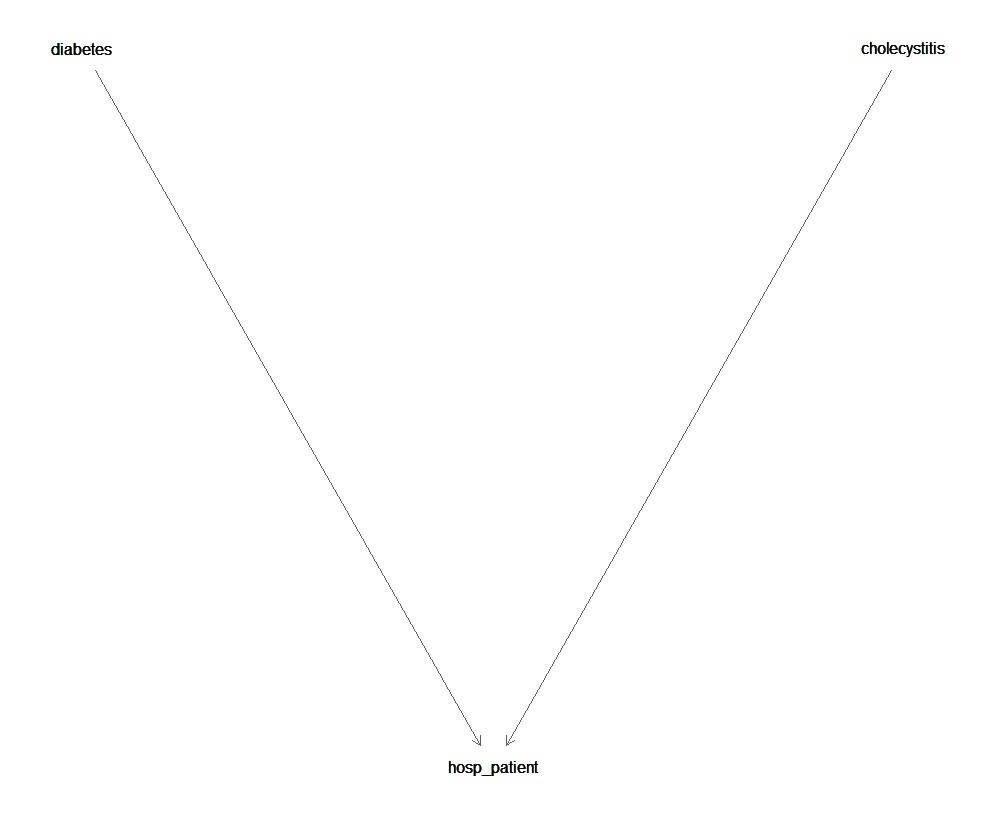
\includegraphics[width=5cm]{BERKS_DAG.png} %%change it for the Berkson one
\centering
\end{figure}
\begin{lstlisting}

Let us generate the data according to the DAG. For this particular case we are going to work with dicotomyc variables.\par

\begin{lstlisting}

N=100

diabetes <- rbinom(n=100, size=1, prob=0.7)
cholecystitis <- rbinom(n=100, size=1, prob=0.3) 
hosp_patients <- diabetes*0.6 + cholecystitis*0.4 + rnorm(N, mean = 0, sd = 0.2)

\end{lstlisting}

Let's take a look at our data estimates, for that we will use a function that creates a dataframe containing the p values and estimates for the variables diabetes and cholecystitis and also diabetes and cholecystitis adjusting by the hospital patients. It also returns a string checking the  significance of the pvalue for diabetes and cholecystitis and another one for the same value but when adjusting by the hospital patients.\par


\begin{lstlisting}

df_pval_estimates <- function(var1, var2, var3) {dataset_2var <- data.frame(var1,var2)

  dataset_3var <- data.frame(var1,var2,var3)
  
  est_v1_v2 <- summary(glm(var1~var2, data = dataset_2var, family = 'binomial')
  )$coefficients['var2', 'Estimate']
  pval_v1_v2 <- summary(glm(var1~var2, data = dataset_2var, family = 'binomial')
  )$coefficients['var2', 'Pr(>|z|)']
  
  est_v1_v2_v3 <- summary(glm(var1~var2+var3, data=dataset_3var, 
                              family = 'binomial'))$coefficients['var2', 'Estimate']
  pval_v1_v2_v3 <-summary(glm(var1~var2+var3, data=dataset_3var, 
                              family = 'binomial'))$coefficients['var2', 'Pr(>|z|)']
  
  df_final <- data.frame('values_of' = c('Estimates', 'P_values'), 'diab_chol' = c(est_v1_v2, pval_v1_v2), 'diab_chol_HP' = c(est_v1_v2_v3, pval_v1_v2_v3))
  
  print(df_final)
  cat('\n')
  
  {if (pval_v1_v2 > 0.05)
    cat('The variables do not show an association. The p value is', 
        pval_v1_v2, 'and the estimate is',est_v1_v2, '\n')
    else
      cat('The variables do show an association. The p value is', 
          pval_v1_v2, 'and the estimate is',est_v1_v2, '\n')}
  
  {if (pval_v1_v2_v3 > 0.05)
    cat('The variables do not show an association when adjusting by the collider. The p value is', 
        pval_v1_v2_v3, 'and the estimate is',est_v1_v2_v3, '\n')
    else
      cat('The variables do show an association when adjusting by the collider. The p value is', 
          pval_v1_v2_v3, 'and the estimate is',est_v1_v2_v3, '\n')}}

df_pval_estimates(diabetes, cholecystitis, hosp_patients)

# values_of diab_chol diab_chol_HP
#1 Estimates 0.6988779  -7.36168368
#2  P_values 0.3038396   0.00373474

# The variables do not show an association. The p value is 0.3038396 and the estimate is 0.6988779 
#The variables do show an association when adjusting by the collider. The p value is 0.00373474 and the estimate is -7.361684

\end{lstlisting}

So, for this example we can see how two variables that should not have any association between them, when adjusting for our collider (a small selection of the population, in this case hospital patients) a negative association arises, meaning you should not find the two diseases in one person.\par


\subsection{Simpson's paradox}

A complex causal phenomenom that has been studied for long is the Simpson's paradox: there is a trend between variables when different groups of data are observed, but when the groups are combined, this trend disappears or is reversed. This paradox is commonly explained as a extreme case of confounding, though some experts argue that this is a oversimplification (Hernan, 2017).\par
One striking example of Simpson's paradox is the low birth-weight paradox. It will also help us to introduce the problem that may involve the unmeasured variables: those events that may affect the causal structure of our model but can't be measured, or that we are not even aware of. This example presents the same issue in any of the following two directed acyclic graphs:
\begin{lstlisting}
LBWsc1.DAG <- dagitty('dag {
Smoking -> LBW
Smoking -> Mortality
U -> LBW
U -> Mortality}')

coordinates(LBWsc1.DAG) <- list(x = c(LBW = 1, Smoking = 2, U = 2, Mortality = 3), y = c(LBW = 3, Smoking = 2, U = 1, Mortality = 3))

drawdag(LBWsc1.DAG)
\end{lstlisting}
\begin{figure}[h]
\caption{Low birth weight paradox as scenario 1.A}
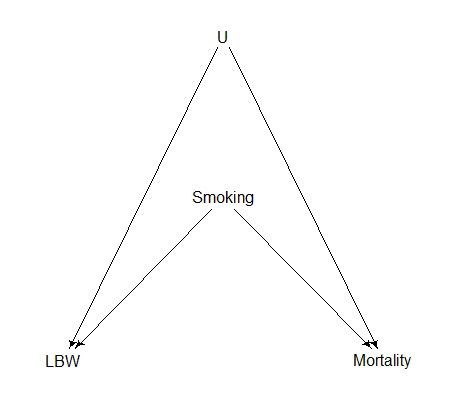
\includegraphics[width=8cm]{LBW1DAG.png}
\centering
\end{figure}
\newpage
\begin{lstlisting}
LBWsc2.DAG <- dagitty("dag {
Smoking -> LBW
LBW -> Mortality
Smoking -> Mortality
U -> LBW
U -> Mortality}")

coordinates(LBWsc2.DAG) <- list(x = c(LBW = 1, Smoking = 2, U = 2, Mortality = 3), y = c(LBW = 3, Smoking = 2, U = 1, Mortality = 3))

drawdag(LBWsc2.DAG)
\end{lstlisting}

\begin{figure}[h]
\caption{Low birth weight paradox as scenario 1.B}
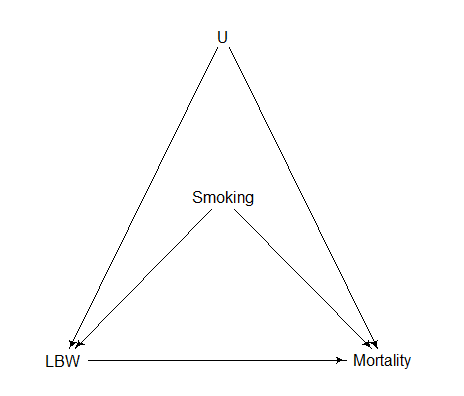
\includegraphics[width=8cm]{LBW2DAG.png}
\centering
\end{figure}
\newpage
The variables of study are three: if the mother smokes or not, if the baby presents a low weight at the moment of birth, and if the baby survives the first month of life. Notice the shape of the graphs: if U is ignored, they are the same scenarios as presented in the common cause section. What medical studies suggest is that underweighted babies present less chances of survival than ordinary babies for multiple reasons: weight involves a better organ development, and indicates that there is certain fat that can be used for protection, warmth and energy. Experts also proclaim that if the mother smokes during the pregnancy, the baby development can be compromised, leading to miscarriage or fragile health (increasing infant mortality). But when 'smoking mother' and 'low birth weight' are implied in the same model, it seems that if the mother smokes during the pregnancy, and the baby has low weight at birth, she has less chances of dying. \par
In this example, there are unmeasured variables (U) that affect both low birth weight and mortality, though the only cause that we are accounting for is smoking. The questions that arise are: does smoking cause mortality? Does low birth weight cause mortality? We will simulate the data with the R package \textbf{simstudy}. We will increase the natural probabilities to visualize with clarity the issue. Let's assume that U is an unkown health condtion that can be absent (0) or present (1).\par
\begin{lstlisting}
samplesize <- 10000
#Data for scenario 1
var.sc1 <- defData(varname = 'U', dist = 'binary', formula = 0.5)
var.sc1 <- defData(var.sc1, varname = 'Smoking', dist = 'binary', formula = 0.5)
var.sc1 <- defData(var.sc1, varname = 'LBW', dist = 'binary', formula = '0.5 * U + 0.4 * Smoking', link = 'identity')
var.sc1 <- defData(var.sc1, varname = 'Mortality', dist = 'binary', formula = '0.05 * Smoking + 0.95 * U', link = 'identity')
set.seed(13)
LBWsc1.df <- genData(samplesize, var.sc1)
#Data for scenario 2
var.sc2 <- defData(varname = 'U', dist = 'binary', formula = 0.5)
var.sc2 <- defData(var.sc2, varname = 'Smoking', dist = 'binary', formula = 0.5)
var.sc2 <- defData(var.sc2, varname = 'LBW', dist = 'binary', formula = '0.5 * U + 0.4 * Smoking', link = 'identity')
var.sc2 <- defData(var.sc2, varname = 'Mortality', dist = 'binary', formula = '0.01 * Smoking + 0.7 * U + 0.1 * LBW', link = 'identity')
set.seed(13)
LBWsc2.df <- genData(samplesize, var.sc2)
\end{lstlisting}

With the following function, we will see what actually happens with the variable Smoking when LBW is present in the model. The coefficients and estimates that are not relevant for the problem are not shown:\par

\begin{lstlisting}
LBW.fun <- function(dataset, reps = 100){
  onlyS_coefS <- rep(NA, reps)
  both_coefS <- rep(NA, reps)
  
  for (i in 1:reps){
    onlyS <- glm(Mortality~Smoking, data = dataset, family = 'binomial')
    both <- glm(Mortality~LBW+Smoking, data = dataset, family = 'binomial')
    
    onlyS_coefS[i] <- summary(onlyS)$coefficients['Smoking','Estimate']
    both_coefS[i] <- summary(both)$coefficients['Smoking','Estimate'] }
  
  cat('\nThe estimate for Smoking is:\nWhen Mortality ~ Smoking:', mean(onlyS_coefS),
      '\nWhen Mortality ~ Smoking + LBW:', mean(both_coefS), '\n')}
      
LBW.fun(LBWsc1.df)
#The estimate for Smoking is:
#When Mortality ~ Smoking: 0.180505 
#When Mortality ~ Smoking + LBW: -0.7805442
LBW.fun(LBWsc2.df)
#The estimate for Smoking is:
#When Mortality ~ Smoking: 0.2600481 
#When Mortality ~ Smoking + LBW: -0.7021735 
\end{lstlisting}

It doesn't matter if in the DAG the variable of low birth weight relates to mortality or not, in both cases when the model conditions on it, the estimate for Smoking gets negative.\footnote{The estimate for Smoking, though not shown, is always significant, as it is directly related to Mortality. This should be obvious up to this point.} These results are contraintuitive: there is something that we are not taking into account.\par
What happens is that those unmeasured variables have a higher influence on mortality and low birth weight than smoking, maybe because they cause serious birth defects. They are 'invisible confounders' that may lead to a wrong conclusion, and by conditioning on Low Birth Weight we are creating a bridge for them to show their effect.\par
It is very common for the so called experts to get excited when they have measured many variables, but sometimes adjusting for other covariates that enable the exposure of a non\-causal relationship can be a real handicap. This is why there is a necessity to stablish a criteria to know what to condition on and what to avoid.\par
\subsection{Backdoor criteria}
The backdoor cirteria is the most common method to condition on covariates, along with frontdoor criteria which is very similar.
We introduce this concept at the end, as it is necessary to know certain basic concepts of the \(Science of Why\) to apply this criteria correctly and with sense.\par
In the backdoor criteria, given a pair of treatment-outcome variables, we should condition on the set of covariates (Z) that:
\begin{itemize} \item Block all the backdoor paths. \item Are not a descendant of the 'treatment', or cause of study, variable.\end{itemize}
We are going to explain this with another example, given the treatment variable is X\_i and the outcome variable is X\_j:\par
\begin{lstlisting}
complex.DAG <- dagitty('dag{
X_1 -> X_3
X_1 -> X_4
X_2 -> X_4
X_2 -> X_5
X_3 -> X_i
X_4 -> X_i
X_4 -> X_j
X_5 -> X_j
X_i -> X_6
X_6 -> X_j}')

coordinates(complex.DAG) <- list(x = c(X_1 =1, X_3 = 1, X_i =1,X_4 = 2, X_6 = 2,X_2 = 3, X_5 = 3, X_j =3),y = c(X_1=1, X_2 = 1, X_3 =2, X_4 = 2, X_5 = 2, X_i = 3, X_6 = 3, X_j =3))

drawdag(complex.DAG)
\end{lstlisting}
\begin{figure}[h]
\caption{How to condition on this DAG?}
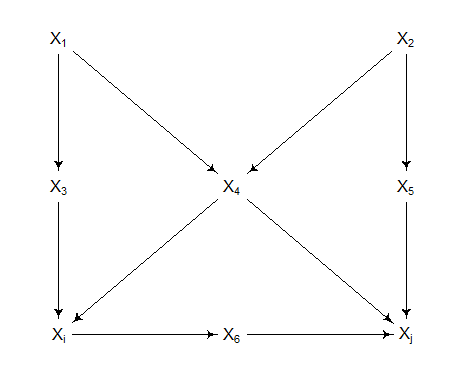
\includegraphics[width=8cm]{complex.DAG.png}
\centering
\end{figure}
First we have to identify all the backdoor paths. A backdoor path is a non causal path between the treatment variable X\_i and the outcome variable, which can be identified by an arrow pointing to X\_i. This can be seen in the following image:\par
\begin{figure}[h]
\caption{Backdoor paths on previous DAG}
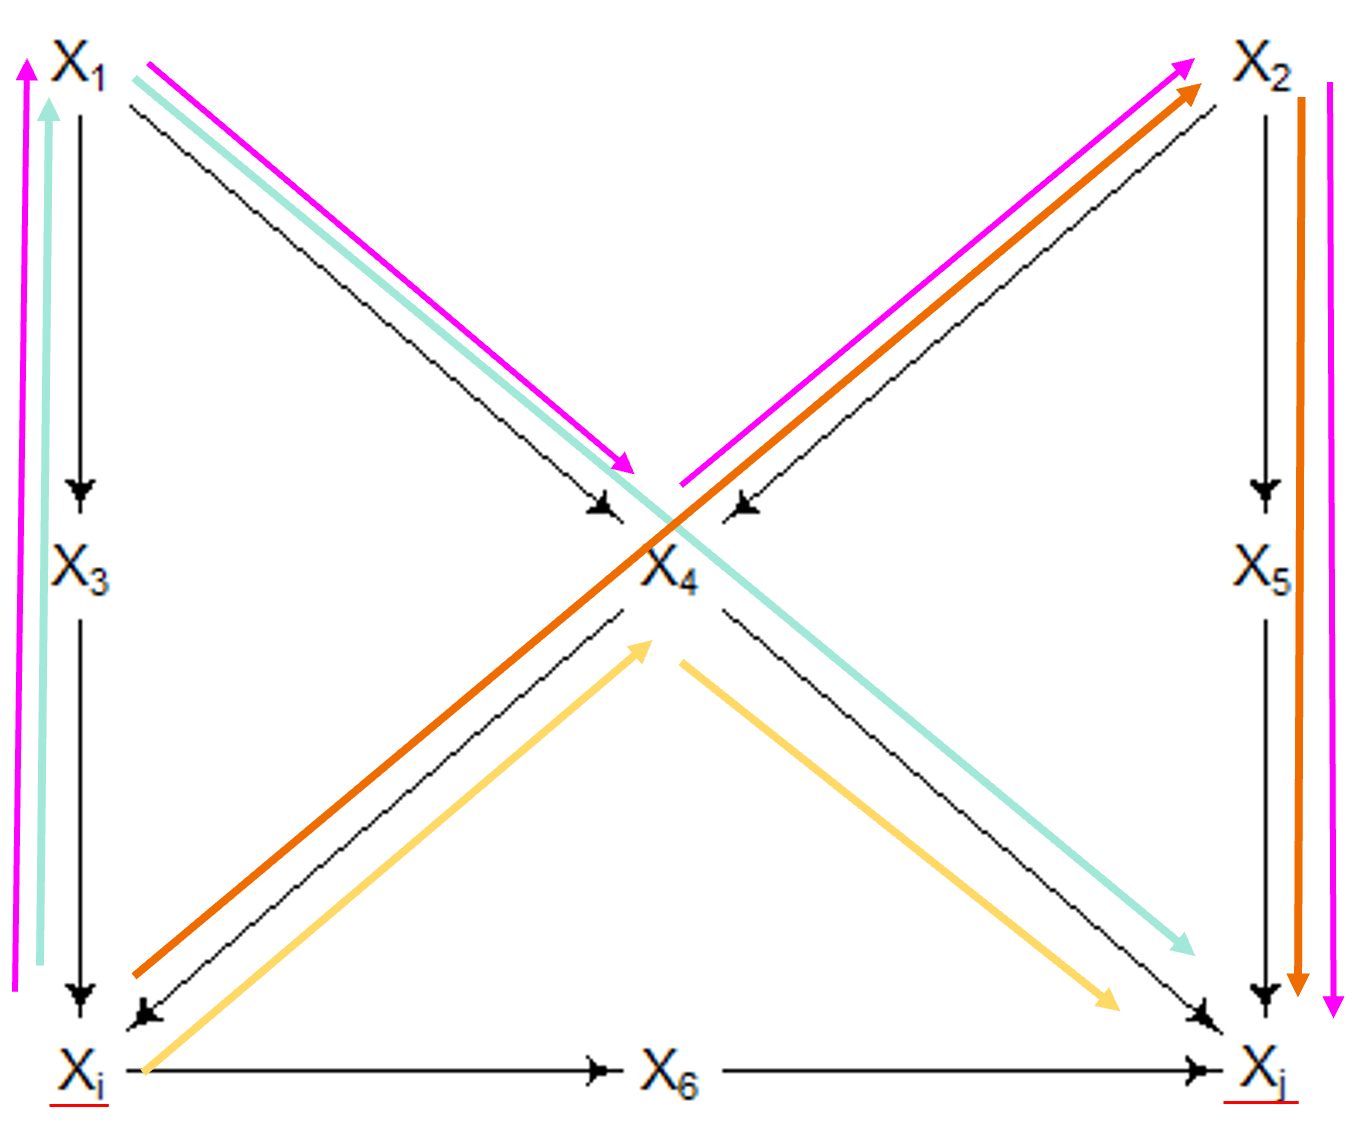
\includegraphics[width=8cm]{complex.DAG.arrows.png}
\centering
\end{figure}
The R package \(dagitty\) contains a function, \(paths\), that can get all the paths between the treatment and the outcome variable. If the graph is too complex, it could be useful to use this package and exclude the causal paths to get the backdoor ones.\par
\begin{lstlisting}
paths(complex.DAG, from = 'X_i', to = 'X_j')$paths
#[1] "X_i -> X_6 -> X_j"                            
#[2] "X_i <- X_3 <- X_1 -> X_4 -> X_j"              
#[3] "X_i <- X_3 <- X_1 -> X_4 <- X_2 -> X_5 -> X_j"
#[4] "X_i <- X_4 -> X_j"                            
#[5] "X_i <- X_4 <- X_2 -> X_5 -> X_j"
\end{lstlisting}
We would have to exclude path \[1\].\par
The next step would be to identify which variables block all the backdoor paths. In this case, it would be X\_4, as it is present in all of them. It satisfies the second condition, as it is not a descendant of the treatment variable X\_i. In this case, X\_4 is not only a confounder of the variables of study; it is also a collider of two other causes. To account for all the possible causes of confounding, it is necessary to also condition either on one of X\_4 parents or on one of the descendants of those parents. The function \(adjustmentSets\) is useful to get all the possible combinations to block these backdoor paths:\par

\begin{lstlisting}
adjustmentSets(complex.DAG, "X_i", "X_j")
#{ X_4, X_5 }
#{ X_2, X_4 }
#{ X_1, X_4 }
#{ X_3, X_4 }
\end{lstlisting}

Let's apply the backdoor criteria with the above examples. \par
Berkson\'s paradox is not due to a bad adjustment, but for a bad selection of the data, so applying these criteria won't solve it.\par
In the low birth weight paradox, as long as the U variables are not measured, it is not possible to adjust on anything else but the \'treatment\' variable \(Smoking\)\: the LBW covariate is a descedant of it, so it doesn\'t comply with the second condition. If we could measure the U variable, and name it as 'birth defects', we would have:\par
\begin{lstlisting}
LBWsc3.DAG <- dagitty("dag {
Smoking -> LBW
LBW -> Mortality
Smoking -> Mortality
Birth.defects -> LBW
Birth.defects -> Mortality}")

coordinates(LBWsc3.DAG) <- list(x = c(LBW = 1.5, Smoking = 1, Birth.defects = 1, Mortality = 3),y = c(LBW = 2, Smoking = 3, Birth.defects = 1, Mortality = 2))

drawdag(LBWsc3.DAG)
\end{lstlisting}

\begin{figure}[h]
\caption{Low birth weight paradox if there are not unmeasured variables}
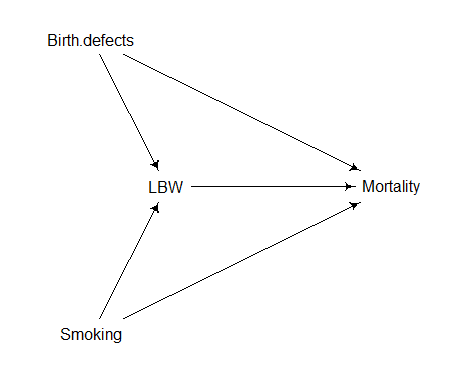
\includegraphics[width=8cm]{LBW3.DAG.png}
\centering
\end{figure}
We can clearly see that it has the same causal structure that another simulation done before, with MATP and INK4a being both descendants of Cortisol and UV radiation. There we concluded that conditioning on both common causes, but not in the mediators, was the best option because their total effect could be appreciated and the variance of the estimates was reduced. Then we explored that conditioning on a collider is not a good idea. Now we can say that the backdoor criteria supports this conclusions. The only backdoor path in this DAG is Smoking, LBW, Birth defects, Mortality. The only option to block it is to condition on birth defects, because LBW is a descendant of Smoking. If we emulate data, and create a function very similar to sc2.comm.extraoverY:\par
\begin{lstlisting}
var.sc3 <- defData(varname = 'Birth_defects', dist = 'binary', formula = 0.5)
var.sc3 <- defData(var.sc3, varname = 'Smoking', dist = 'binary', formula = 0.5)
var.sc3 <- defData(var.sc3, varname = 'LBW', dist = 'binary', formula = '0.5 * Birth_defects + 0.4 * Smoking', link = 'identity')
var.sc3 <- defData(var.sc3, varname = 'Mortality', dist = 'binary', formula = '0.1 * Smoking + 0.7 * Birth_defects + 0.1 * LBW', link = 'identity')

set.seed(13)
LBWsc3.df <- genData(samplesize, var.sc3)

LBW.fun_noU <- function(dataset){
  onlyS <- glm(Mortality~Smoking, data = dataset, family = 'binomial')
  onlyBD <- glm(Mortality~Birth_defects, data = dataset, family = 'binomial')
  both <- glm(Mortality~Smoking+Birth_defects, data = dataset, family = 'binomial')
  
  cat('\nThe estimate for Smoking is:\nWhen Mortality ~ Smoking:', 
      summary(onlyS)$coefficients['Smoking','Estimate'],'\ns.d:', 
      summary(onlyS)$coefficients['Smoking','Std. Error'],
      '\nWhen Mortality ~ Smoking + Birth defects:', 
      summary(both)$coefficients['Smoking','Estimate'], '\ns.d:', 
      summary(both)$coefficients['Smoking','Std. Error'],'\n')
  cat('\nThe estimate for Birth defects is:\nWhen Mortality ~ Smoking:', 
      summary(onlyBD)$coefficients['Birth_defects','Estimate'],'\ns.d:', 
      summary(onlyBD)$coefficients['Birth_defects','Std. Error'],
      '\nWhen Mortality ~ Smoking + Birth defects:', 
      summary(both)$coefficients['Birth_defects','Estimate'], '\ns.d:', 
      summary(both)$coefficients['Birth_defects','Std. Error'],'\n')}

LBW.fun_noU(LBWsc3.df)

#The estimate for Smoking is:
#When Mortality ~ Smoking: 0.2600481 
#s.d: 0.4063957 
#When Mortality ~ Smoking + Birth defects: 0.9710298 
#s.d: 0.6415113 

#The estimate for Birth defects is:
#When Mortality ~ Smoking: 3.819908 
#s.d: 0.6301974 
#When Mortality ~ Smoking + Birth defects: 4.041328 
#s.d: 0.684317 
\end{lstlisting}
The paradox has been neutralised: the effect of Smoking on Mortality isn't negative when we adjust on the covariate Birth Defects. \footnote{It gets slightly higher, as well as its variance. We would need to do more trials and experiments to understand what is going on, which goes beyond the scope of this project.} Smoking increases Mortality though Birth Defects have a bigger effect.\par
\newpage
\section{Conclusion}

As we have seen, causal inference analysis have more tricks and traps than expected. It is crucial to know the causal structure that is followed in the real life cases, and use it properly. If this first model is not correct, it will be very difficult to have a correct insight of the problem. For this same reason, we cannot forget the causal context of the covariates and reduce them just to scatistical terms. The causal structure is important if we want to apply backdoor criteria, and to identify if what we are observing is a direct effect or a total effect. 


\section{References}

Causal Mediation | Columbia Public Health. (2022). Retrieved 11 January 2022, from \href{https://www.publichealth.columbia.edu/research/population-health-methods/causal-mediation}{PublicHealth Columbia - Causal Mediation}

Coffman, D., \& Zhong, W. (2012). Assessing mediation using marginal structural models in the presence of confounding and moderation. Psychological Methods, 17(4), 642-664. doi: 10.1037\/a0029311

Cole, S., \& Hernan, M. (2002). Fallibility in estimating direct effects. International Journal Of Epidemiology, 31(1), 163-165. doi: 10.1093\/ije\/31.1.163

Davis, D. (2020). Average Sprinting Speed \& Usain Bolt Top Speed | Track Spikes. Retrieved 11 January 2022, from \href{https://trackspikes.co.uk/average-sprinting-speed/#}{Trackspikes.co.uk}

Hernan, M. (2017). Simpson's Paradox Unraveled. Retrieved 11 January 2022, from \href{https://twitter.com/_MiguelHernan/status/860542619818106881?s=20}{Miguel Hernan's Tweet, very recomended blog.}

Hernan, M., Clayton, D., \& Keiding, N. (2011). The Simpson\'s paradox unraveled. International Journal Of Epidemiology, 40(3), 780\-785. doi: 10.1093\/ije\/dyr041

Santalo Bel, M., Guindo Soldevila, J., \& Ordonez Llanos, J. (2003). Marcadores biológicos de necrosis miocardica. Revista Española De Cardiologia, 56(7), 703-720. doi: 10.1016\/s0300-8932(03)76942-5

SARS-CoV-2: PCR, Carga Viral y CTs | Life Length BLOG (2022). Retrieved 11 January 2022, \href{from https://lifelength.com/es/sars-cov-2-pcr-carga-viral-y-cts/}{Life Length Divulgation Blog}

Soufir, N., Guedj, M., Bourrillon, A., Combadieres, C., Descamps, V., \& Dupin, N. et al. (2008). Polymorphisms of the MATP\/SLC45A2 gene and susceptibility to melanoma in the French population. Journal Of Clinical Oncology, 26(15\_suppl), 11040-11040. doi: 10.1200\/jco.2008.26.15\_suppl.11040

The Birth-Weight paradox. Retrieved 11 January 2022, from \href{https://library.bayesia.com/articles/#!bayesialab-knowledge-hub/the-birth-weight-paradox}{BayesiaLab - Weight Paradox simulation}

Cholesterol Levels: What You Need to Know: MedlinePlus. Retrieved 11 January 2022, from \href{https://medlineplus.gov/cholesterollevelswhatyouneedtoknow.html}{MedlinePlus.gov}

Troponin - Health Encyclopedia - University of Rochester Medical Center. Retrieved 11 January 2022, from \href{https://www.urmc.rochester.edu/encyclopedia/content.aspx?contenttypeid=167&contentid=troponin}{Encyclopedia entry: Troponin}

VanderWeele, T. (2014). Commentary: Resolutions of the birthweight paradox: competing explanations and analytical insights. International Journal Of Epidemiology, 43(5), 1368-1373. doi: 10.1093\/ije\/dyu162

VanderWeele, T., \& Shpitser, I. (2011). A New Criterion for Confounder Selection. Biometrics, 67(4), 1406-1413. doi: 10.1111\/j.1541-0420.2011.01619.x

\end{document}
